\section{Results}\label{sec:results} 

In this section, we describe the results of our experiments.  We explore which
non-mainstream resolvers are available; how
the performance of mainstream resolvers compares to that of non-mainstream
resolvers; and whether (and to what extent) encrypted DNS response time
correlates to high network latency. As described
in Section~\ref{sec:method}, our results represent measurements
from October 2021; future work could perform ongoing
measurements based on the measurement framework we have developed to validate
and extend these results.

\subsection{Are Non-Mainstream Resolvers Available?}

\if 0
\begin{table}[t!]
\centering
\begin{tabular}{lllll}
\hline
\textbf{Location} & \textbf{Resolver} & \textbf{Responsive?} & & \\
    & & \textbf{Ohio} & \textbf{Seoul} & \textbf{Frankfurt} \\
\midrule
North America     & \begin{tabular}[c]{@{}l@{}}dnscrypt.ca-1-doh\\ dnscrypt.ca-2-doh\\ doh-cleanbrowsing\\ doh.post-factum.tk\end{tabular} & \begin{tabular}[c]{@{}l@{}}\\ \\ \\ \end{tabular} & \begin{tabular}[c]{@{}l@{}}\\ \\ \\ \end{tabular} & \begin{tabular}[c]{@{}l@{}}\\ \\ \\ \end{tabular}    \\ \midrule
Asia              & \begin{tabular}[c]{@{}l@{}}doh.tiarap.org\\ jp.tiarap.org\\ doh.linuxsec\end{tabular} & \begin{tabular}[c]{@{}l@{}}\\ \\ \end{tabular}      & \begin{tabular}[c]{@{}l@{}}\\ \\ \end{tabular}      & \begin{tabular}[c]{@{}l@{}}\checkmark\ \checkmark\ \end{tabular}            \\ \midrule
Europe            & \begin{tabular}[c]{@{}l@{}}doh.bortzmeyer\\ doh.appliedprivacy\\ doh.chewbacca.meganerd.nl\\ doh.powerdns\end{tabular} & \begin{tabular}[c]{@{}l@{}}\\ \\ \\ \end{tabular} & \begin{tabular}[c]{@{}l@{}}\\ \\ \\ \end{tabular} & \begin{tabular}[c]{@{}l@{}}\\ \\ \\ \end{tabular} \\ \bottomrule
\end{tabular}
\caption{Resolvers that failed to respond from each vantage point.}
\label{tab:unresponsive}
\end{table}
\fi


\begin{table}[t!]
\centering
\begin{small}
\begin{tabular}{l|rr}
    \toprule
    \textbf{Error} & \textbf{Count} & \textbf{\% of All Responses} \\
    \midrule
    Couldn't Connect to Server & 47,377 & 7\% \\
    HTTP Error Status & 38,475 & 5.7\% \\
    Couldn't Decode Response & 26,686 & 4\% \\
    SSL Connect Error & 17,720 & 2.6\% \\
    Couldn't Resolve the Resolver's Domain Name & 8,864 & 1.3\% \\
    SSL Certificate Error & 4,465 & 0.7\% \\
    Other Error & 234 & $<$ 1\% \\
    SSL Timeout & 27 & $<$ 1\% \\
    Error in the HTTP/2 Framing Layer & 2 & $<$ 1\% \\
    \midrule
    \textbf{Successful Responses} & \textbf{531,528} & \textbf{78.7\%} \\
    \textbf{All Errors} & \textbf{143,848} & \textbf{21.3\%} \\
    \bottomrule
\end{tabular}
\end{small}
\caption{Errors when trying to perform DoH queries from all vantage points.}
\label{tab:errors}
\end{table}

We first aimed to study the availability of encrypted DNS
resolvers. 
We received responses from most resolvers that we queried.  Table~\ref{tab:errors}
shows the most common errors we received from attempting to communicate with
the resolvers.\footnote{Due to a bug, we did not record one rare error type.}
The most common errors from unavailable resolvers were related
to a failure to establish a TCP connection and a TLS session.  It is likely
that in many of these cases, the resolver itself was simply no longer
operational; additional longitudinal measurements could confirm this
hypothesis.  We did not receive a response from eleven resolvers:
\texttt{dns1.dnscrypt.ca, dns2.dnscrypt.ca, doh.cleanbrowsing.org,
doh.post-factum.tk, doh.linuxsec.org, doh.tiar.app, jp.tiar.app,
doh.appliedprivacy.net, doh.bortzmeyer.fr, doh.chewbacca.meganerd.nl,
doh.powerdns.org}. However, we only performed measurements at a single point
in time, and thus we lack enough measurements to draw general conclusions
about the availability of these resolvers. Future work could extend this work
to perform longitudinal measurements of availability of these
resolvers.\footnote{We will release our measurement framework and data upon
publication of this work.}


\begin{figure}[t!]
\hspace*{-1in}
\begin{minipage}{1.35\textwidth}
    \subfigure[North America (Local).]{%
\label{fig:Ohio_NA}%
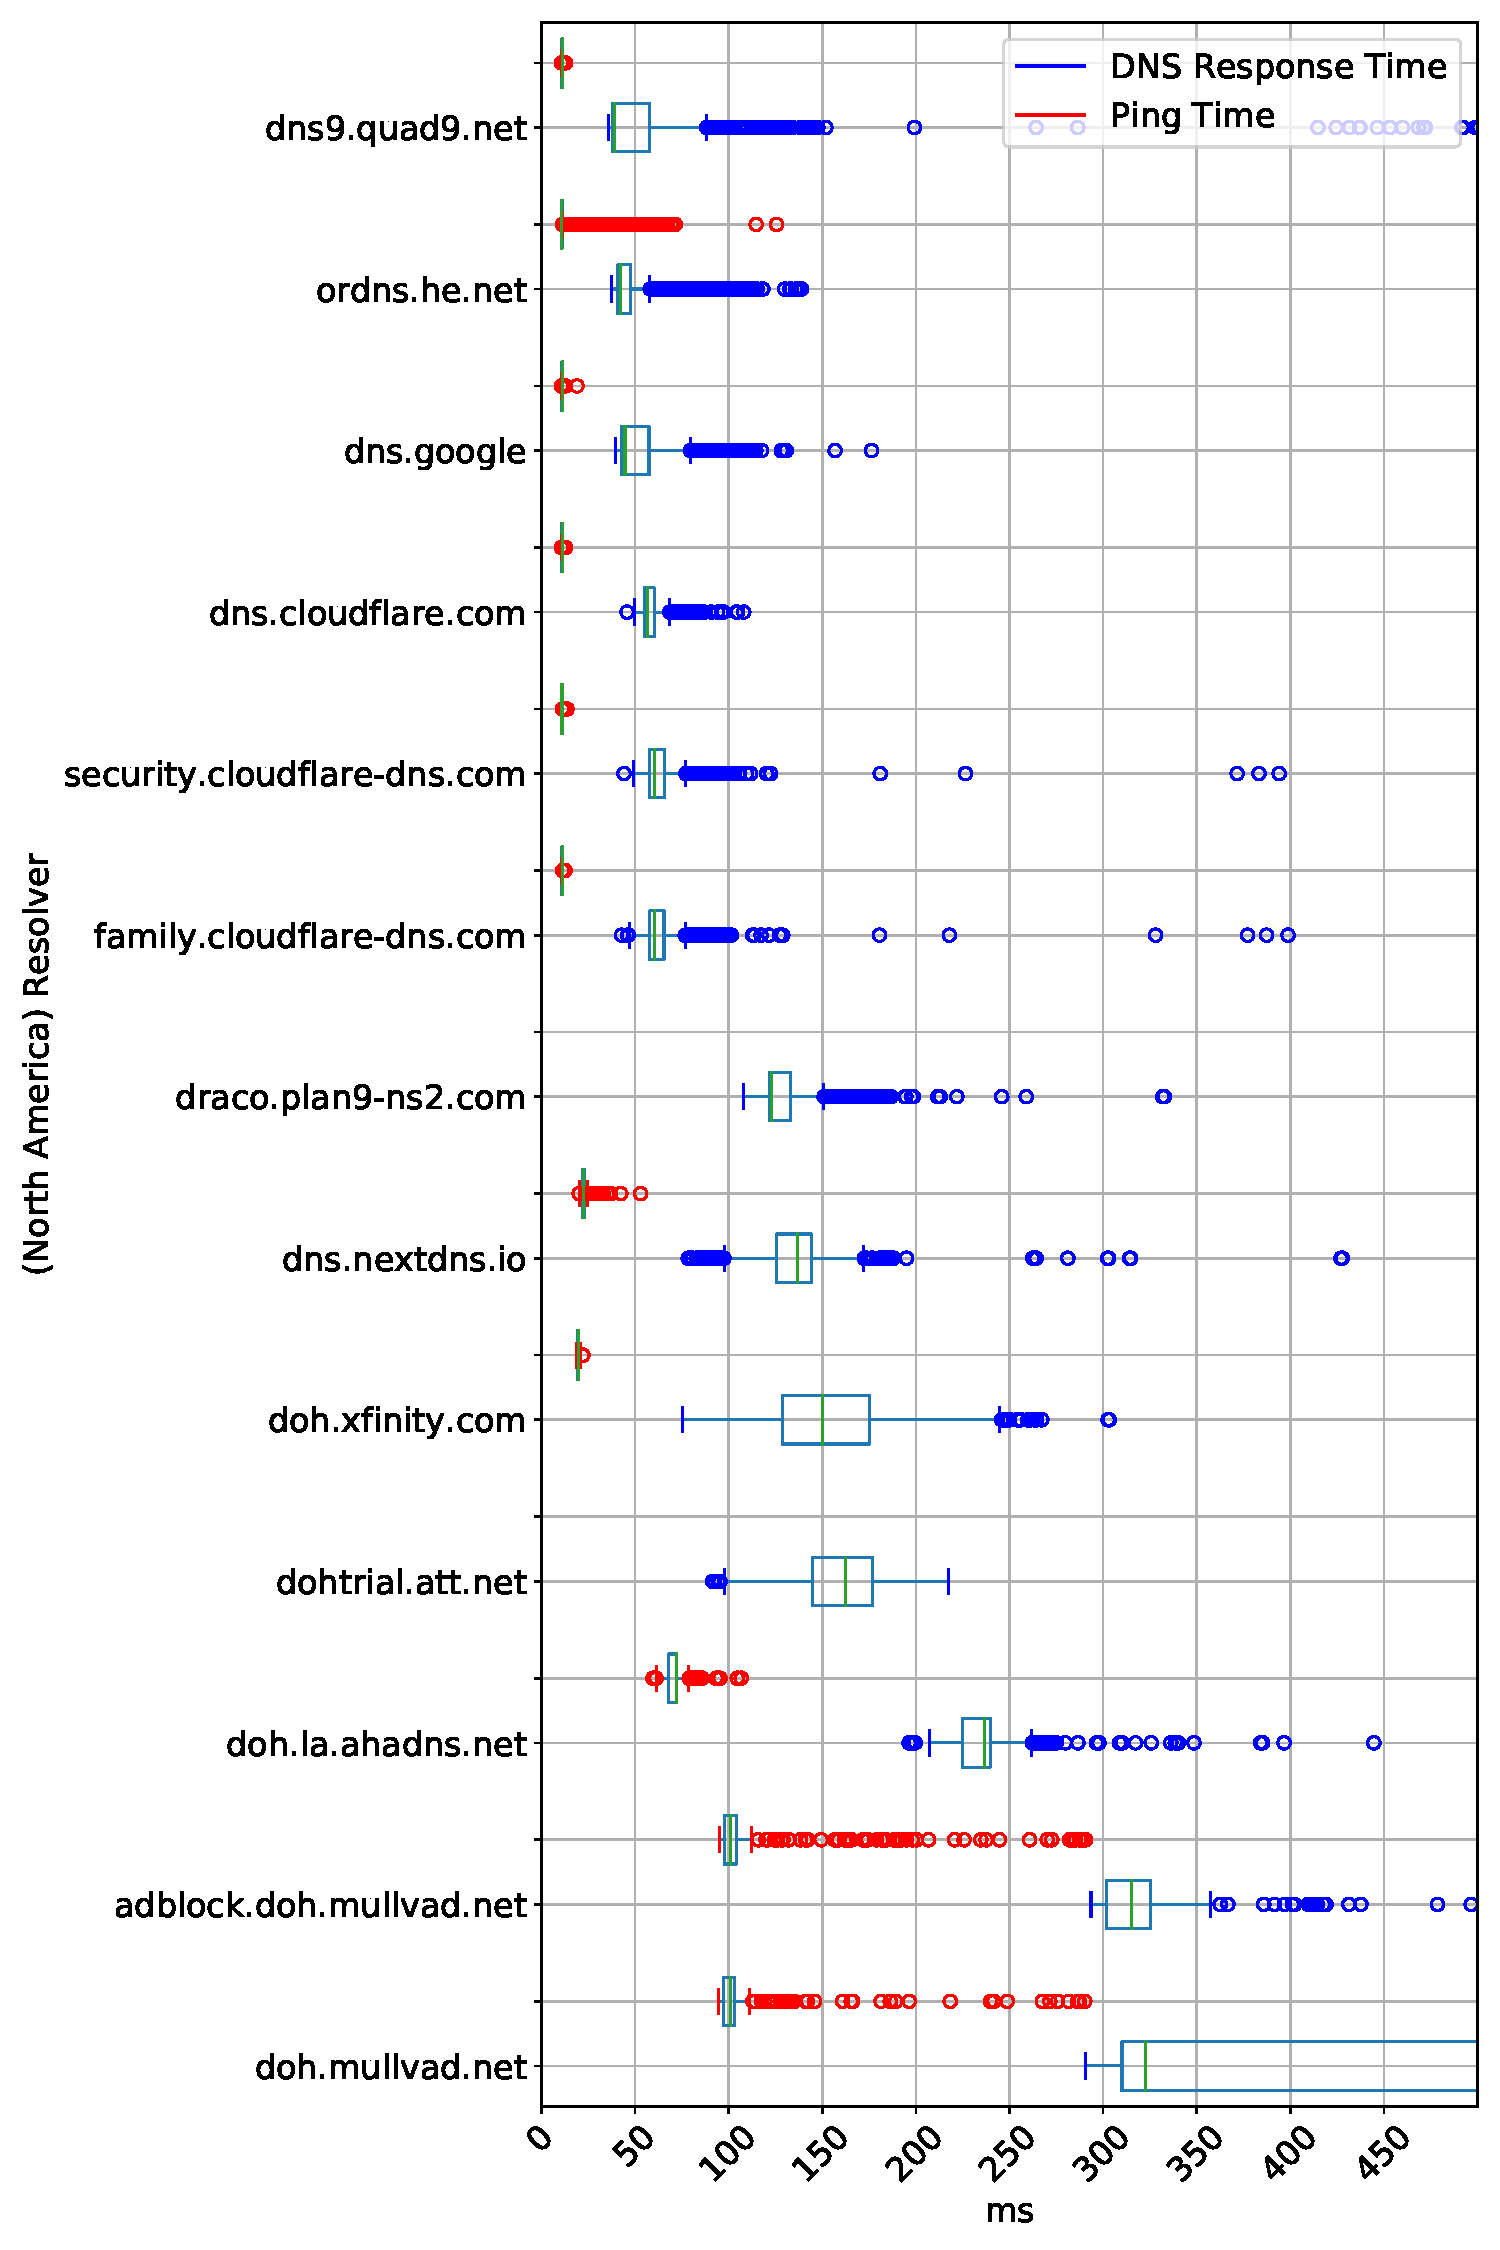
\includegraphics[width=0.32\linewidth]{figures/Ohio_North_America.pdf}}%
\hfill%
\subfigure[Asia.]{%
\label{fig:Ohio_Asia}%
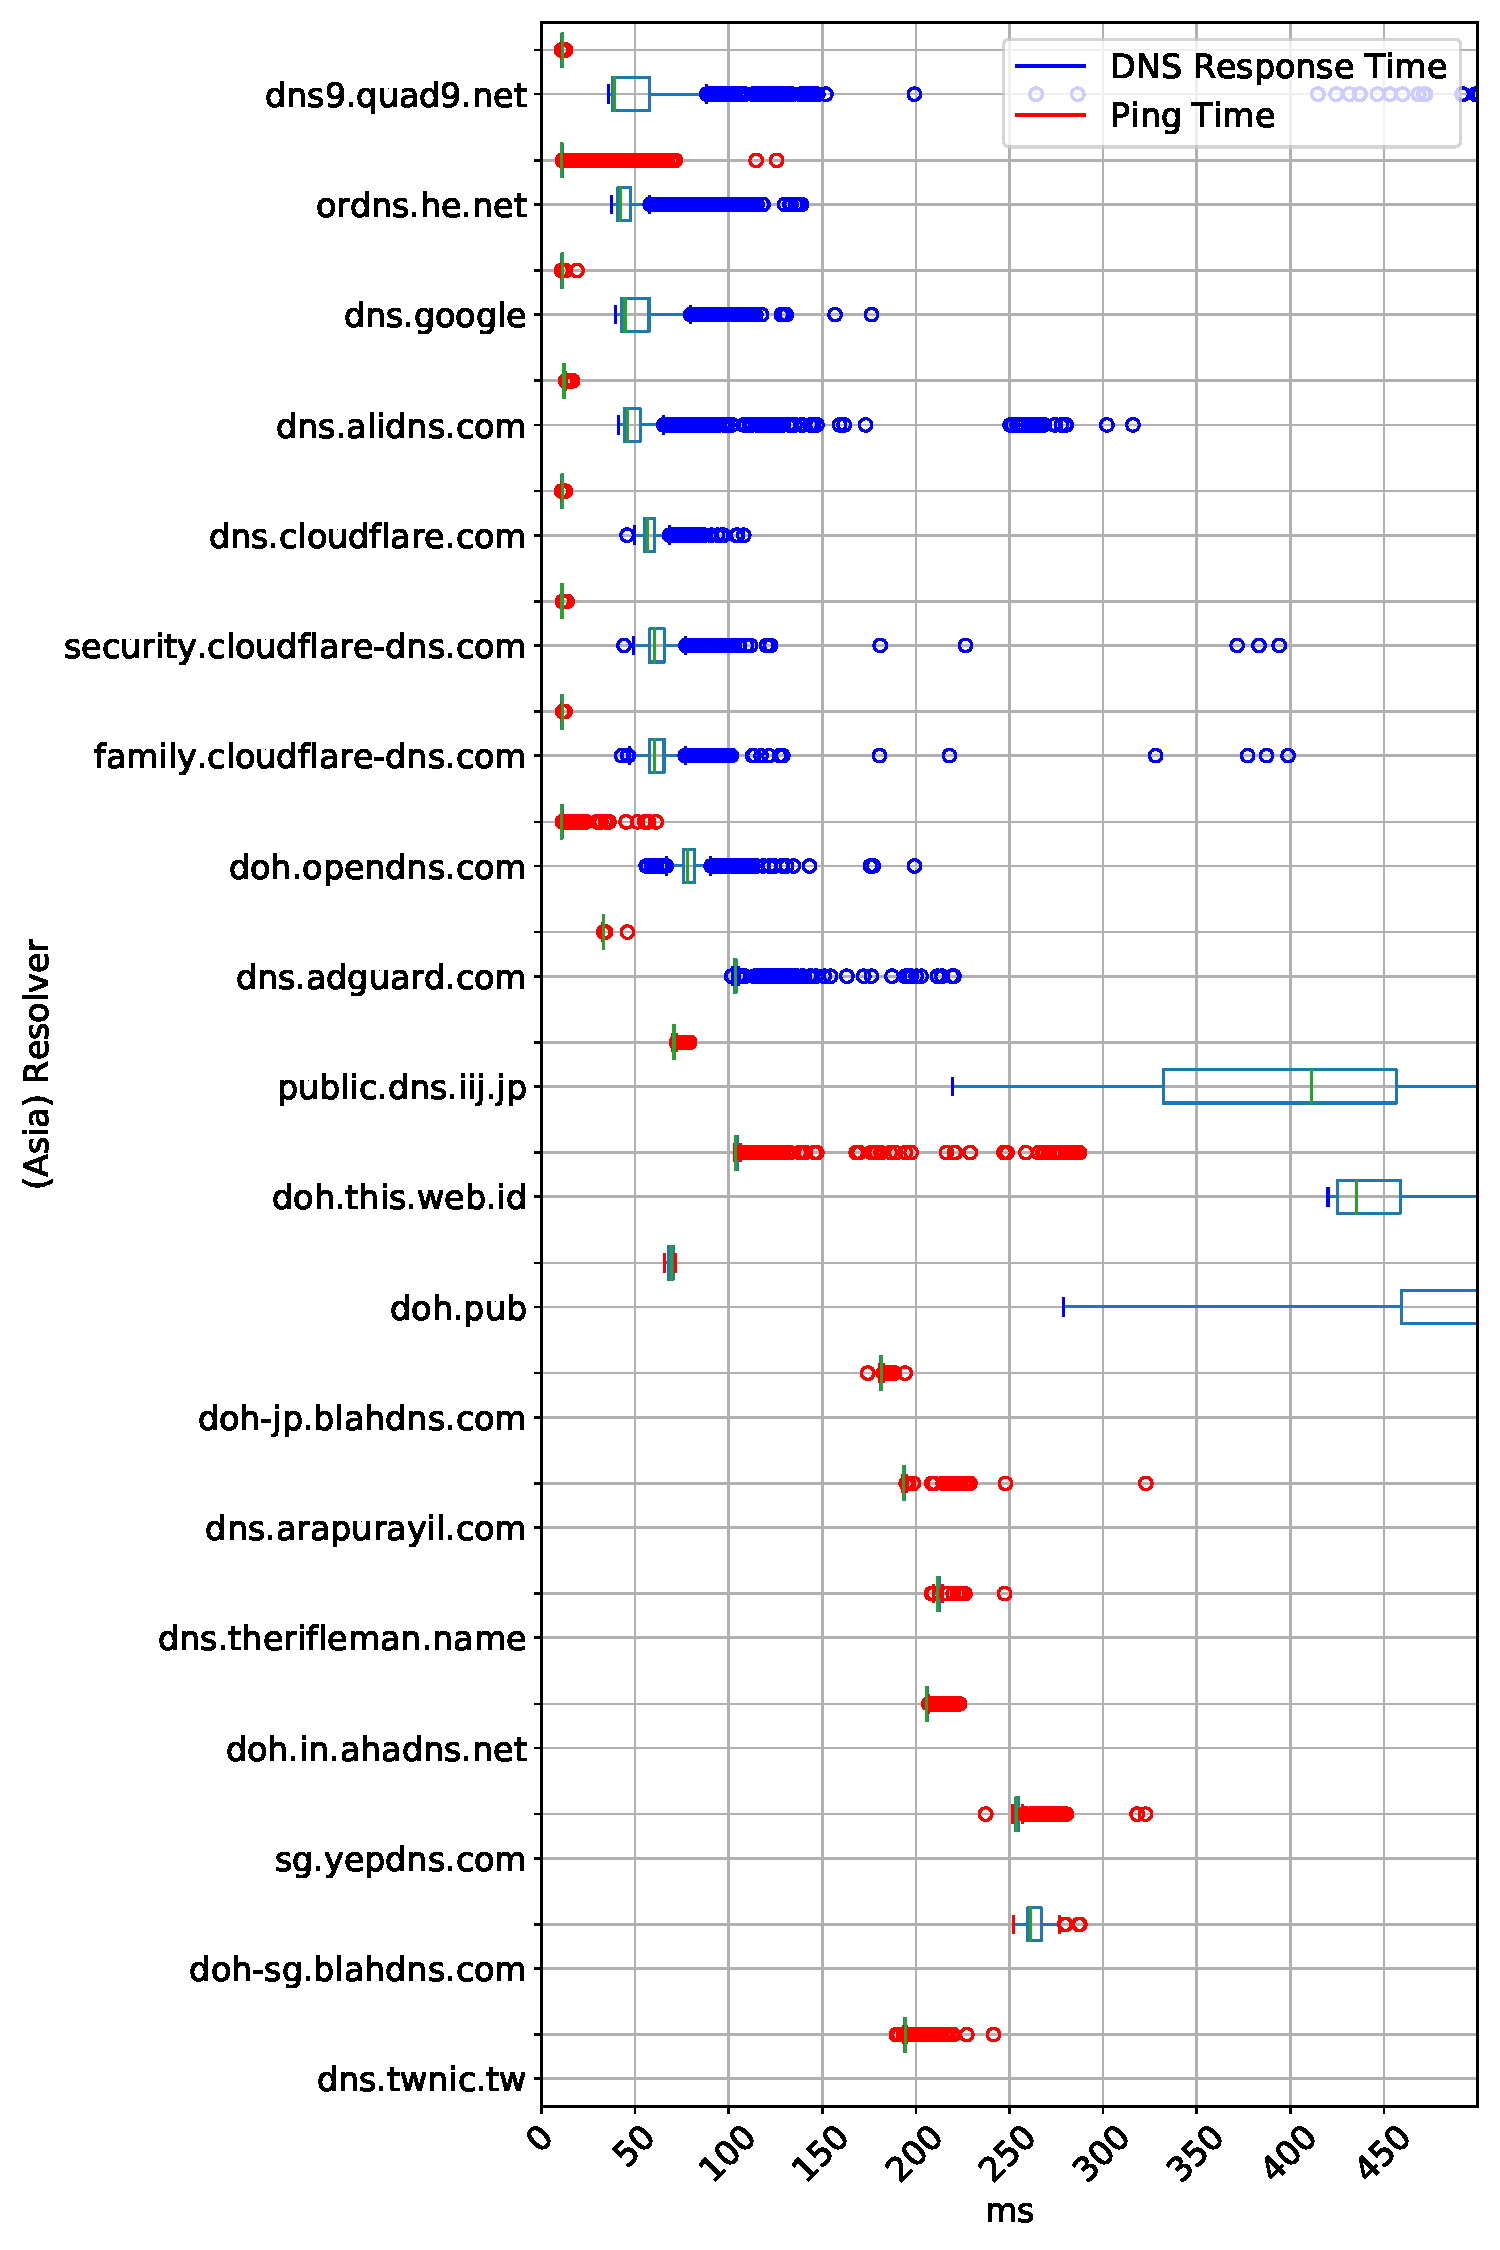
\includegraphics[width=0.32\linewidth]{figures/Ohio_Asia.pdf}}%
\hfill%
\subfigure[Europe.]{%
\label{fig:Ohio_Europe}%
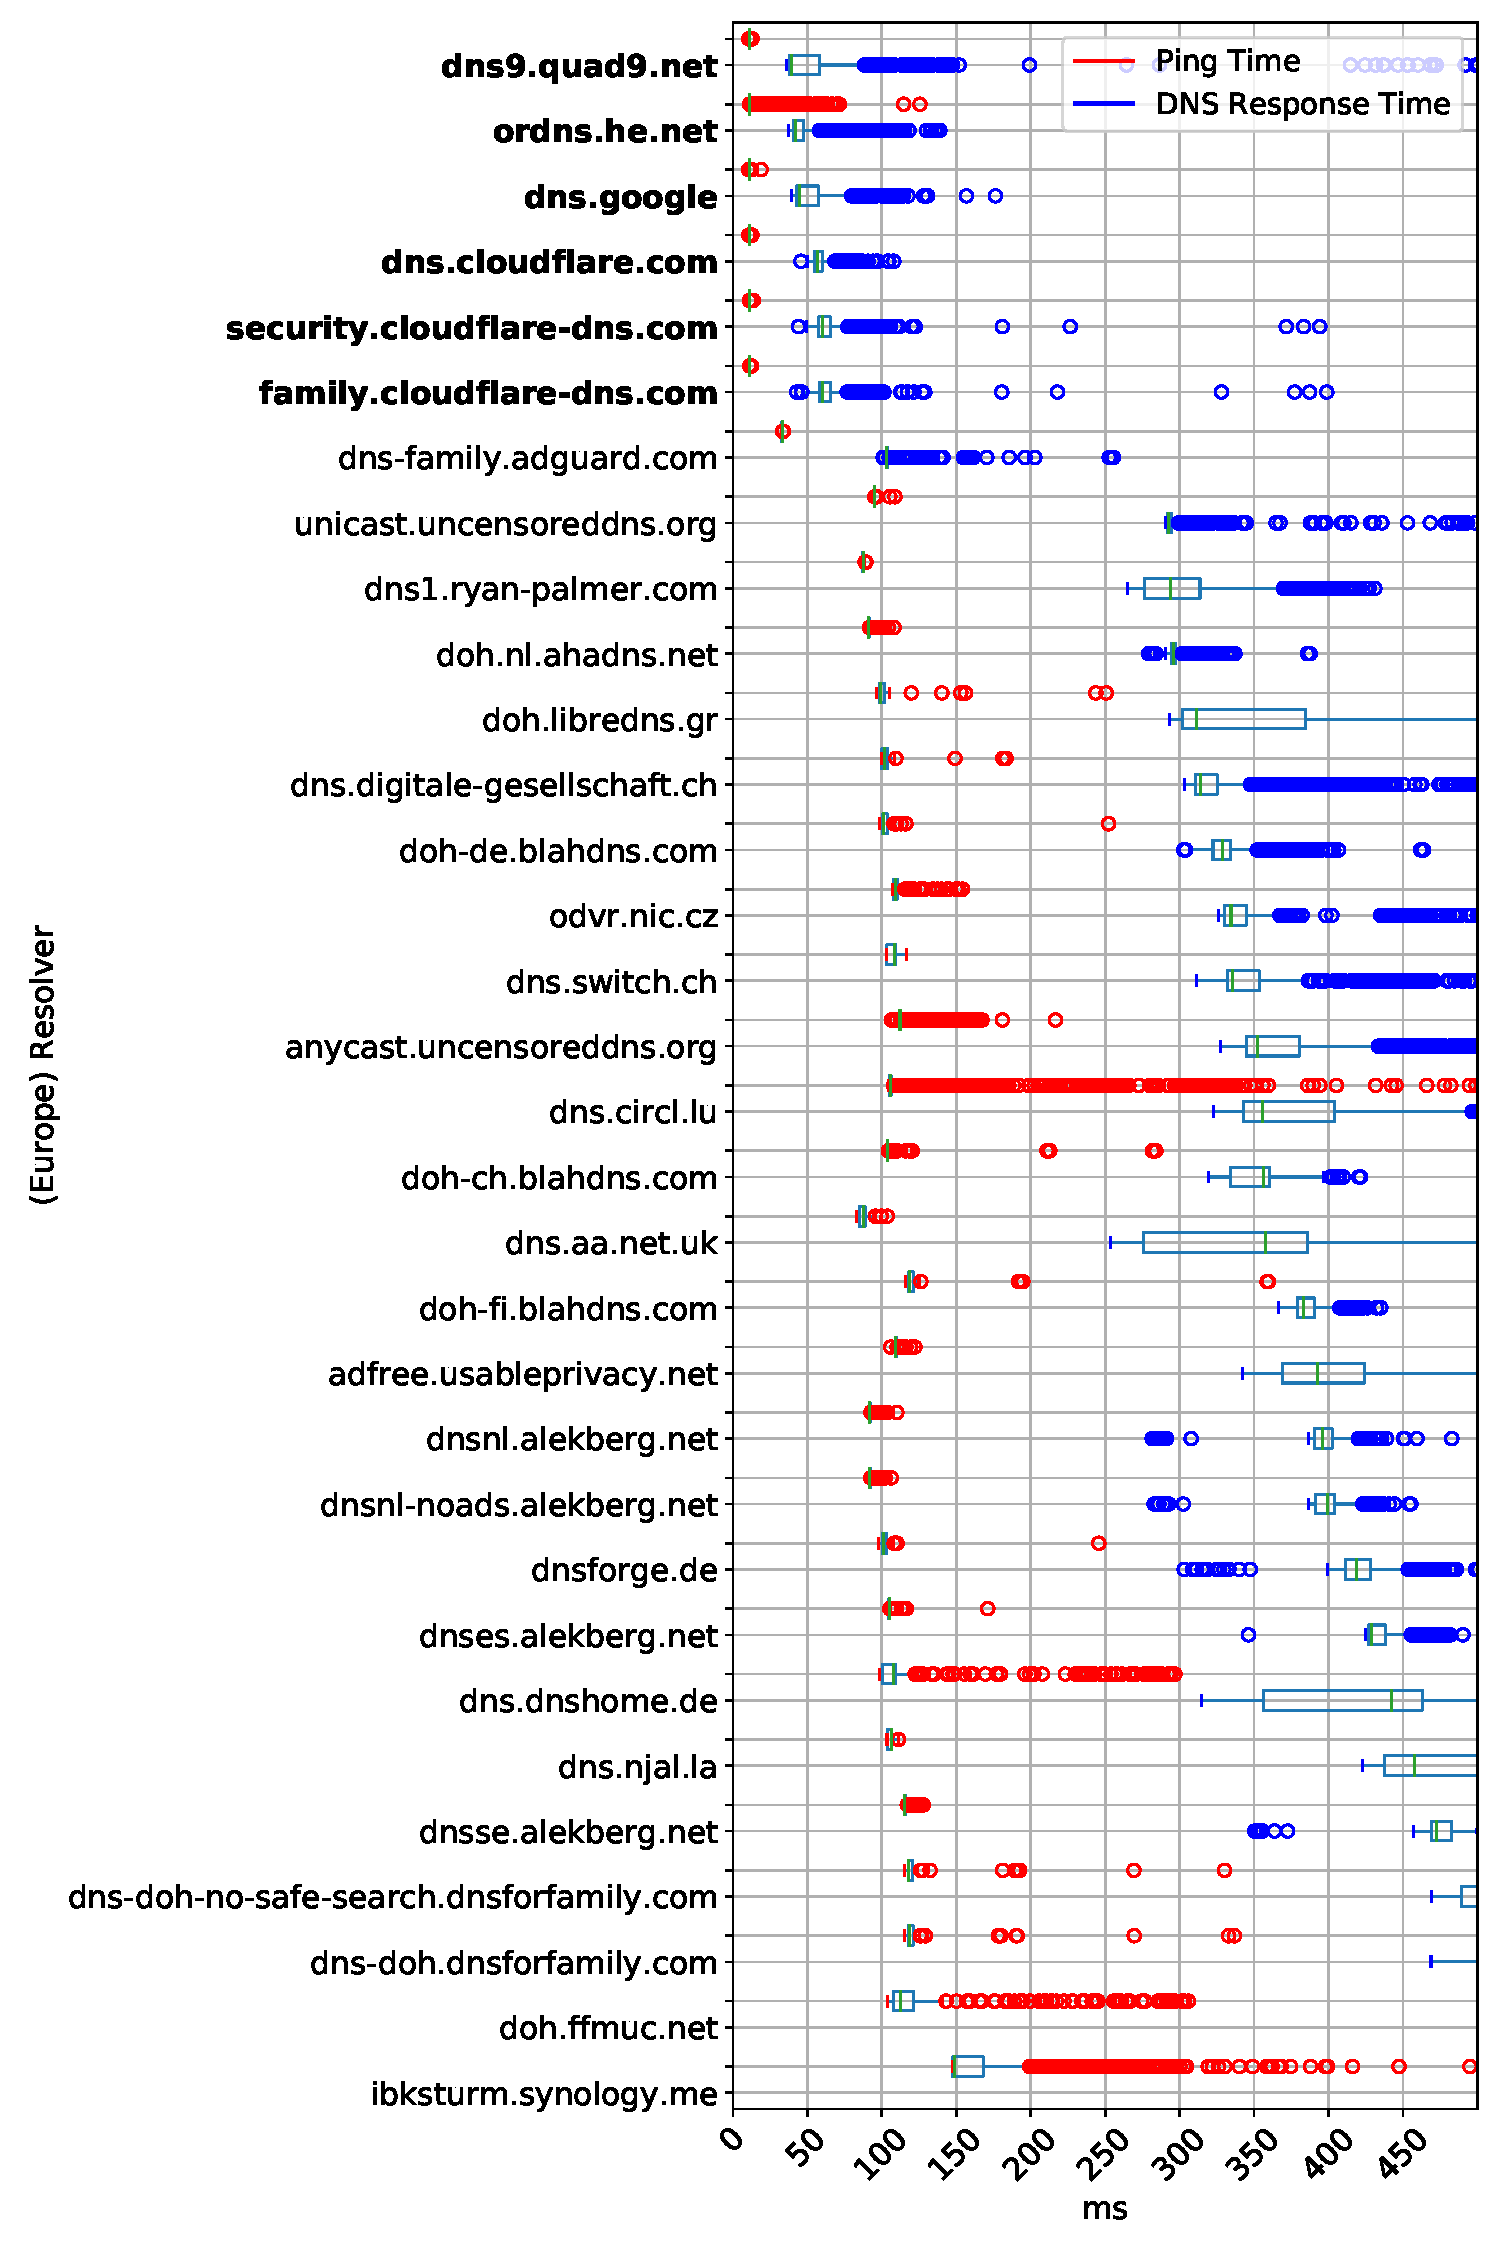
\includegraphics[width=0.32\linewidth]{figures/Ohio_Europe.pdf}}%
    \caption{The DNS response time and ICMP ping time distributions for
    encrypted DNS resolvers measured from a vantage point in the United States
    (Ohio). Mainstream resolvers are shown in boldface across all three
    sub-figures.}
\label{fig:dns-us}
\end{minipage}
\end{figure}

\subsection{\mbox{How Do Non-Mainstream Resolvers Perform?}}

Given the large number of non-mainstream resolvers that have not been
previously studied, we aimed to study how
the performance of these encrypted DNS resolvers compared to mainstream ones.
As previously mentioned, one of our motivations in doing so is to better
understand the global extent of encrypted DNS resolver deployment, as existing
lists of public encrypted DNS resolvers~\cite{dnscrypt-public-resolvers} do
not provide any overview of either reliability or performance. Additionally,
given that most organizations who have deployed mainstream resolvers are based
in the United States, we also wanted to explore how the performance of a
broader set of encrypted DNS resolvers varied by geography.

Figures~\ref{fig:dns-us}--\ref{fig:dns-europe} show the distributions of DNS
response times and ICMP ping times across encrypted DNS resolvers, as measured
from vantage points in the United States, Asia, and Europe, respectively. The
plots show distributions for both DNS response times and ICMP round-trip latency. 
Although some distributions extend beyond 500~ms, we have truncated the plots
for ease of exposition, since responses beyond this range will not result in
good application performance.
Certain resolvers did not respond to our ICMP ping probes; for those
resolvers, no latency data is shown.


As expected, most mainstream resolvers outperformed non-mainstream resolvers
from most vantage points.
Non-mainstream resolvers also exhibited higher variability of 
median query response times.  
From North America, we observe that aside from the five resolvers with the
lowest encrypted DNS response time,
median query response times ranged from 
60~ms to 323~ms, all considerably above typical DNS lookup response times. From Asia, median response times outside
of the top five were extremely variable, ranging from 114~ms to 31.6~seconds. 
Although the slowest resolver in Asia as measured from Asia was an extreme
outlier, we saw that several resolvers in Asia had slow median response times,
even when queried from Asia. For example,
the second-slowest resolver also exhibited slow performance, with a median
response time of about one second from our vantage point in Asia.
We observe more
consistent performance for resolvers in Europe, but we still
see median query response times outside the top five range from 19 ms to
156 ms.

In some cases, however, a particular non-mainstream resolver would outperform
the mainstream DoH resolvers.  As expected, \texttt{dns.quad9.net},
\texttt{dns.google}, and \texttt{dns.cloudflare.com} were among the top five
highest performing DoH resolvers in North America, Europe, and Asia.
Interestingly, however, \texttt{ordns.he.net}---a DoH resolver hosted by
Hurricane Electric, a global Internet service provider (ISP)---managed to
outperform \texttt{dns.google} and \texttt{dns.cloudflare.com} from all three
vantage points.  From Frankfurt, \texttt{dns-family.adguard.com} and
\texttt{ordns.he.net} are the top two highest performing resolvers; from
Seoul, \texttt{doh-jp.blahdns.com} and \texttt{ordns.he.net} outperforms \texttt{dns.google}.

\begin{figure}[t!]
\hspace*{-1in}
\begin{minipage}{1.35\textwidth}
\centering
\subfigure[North America.]{%
\label{fig:Seoul_NA}%
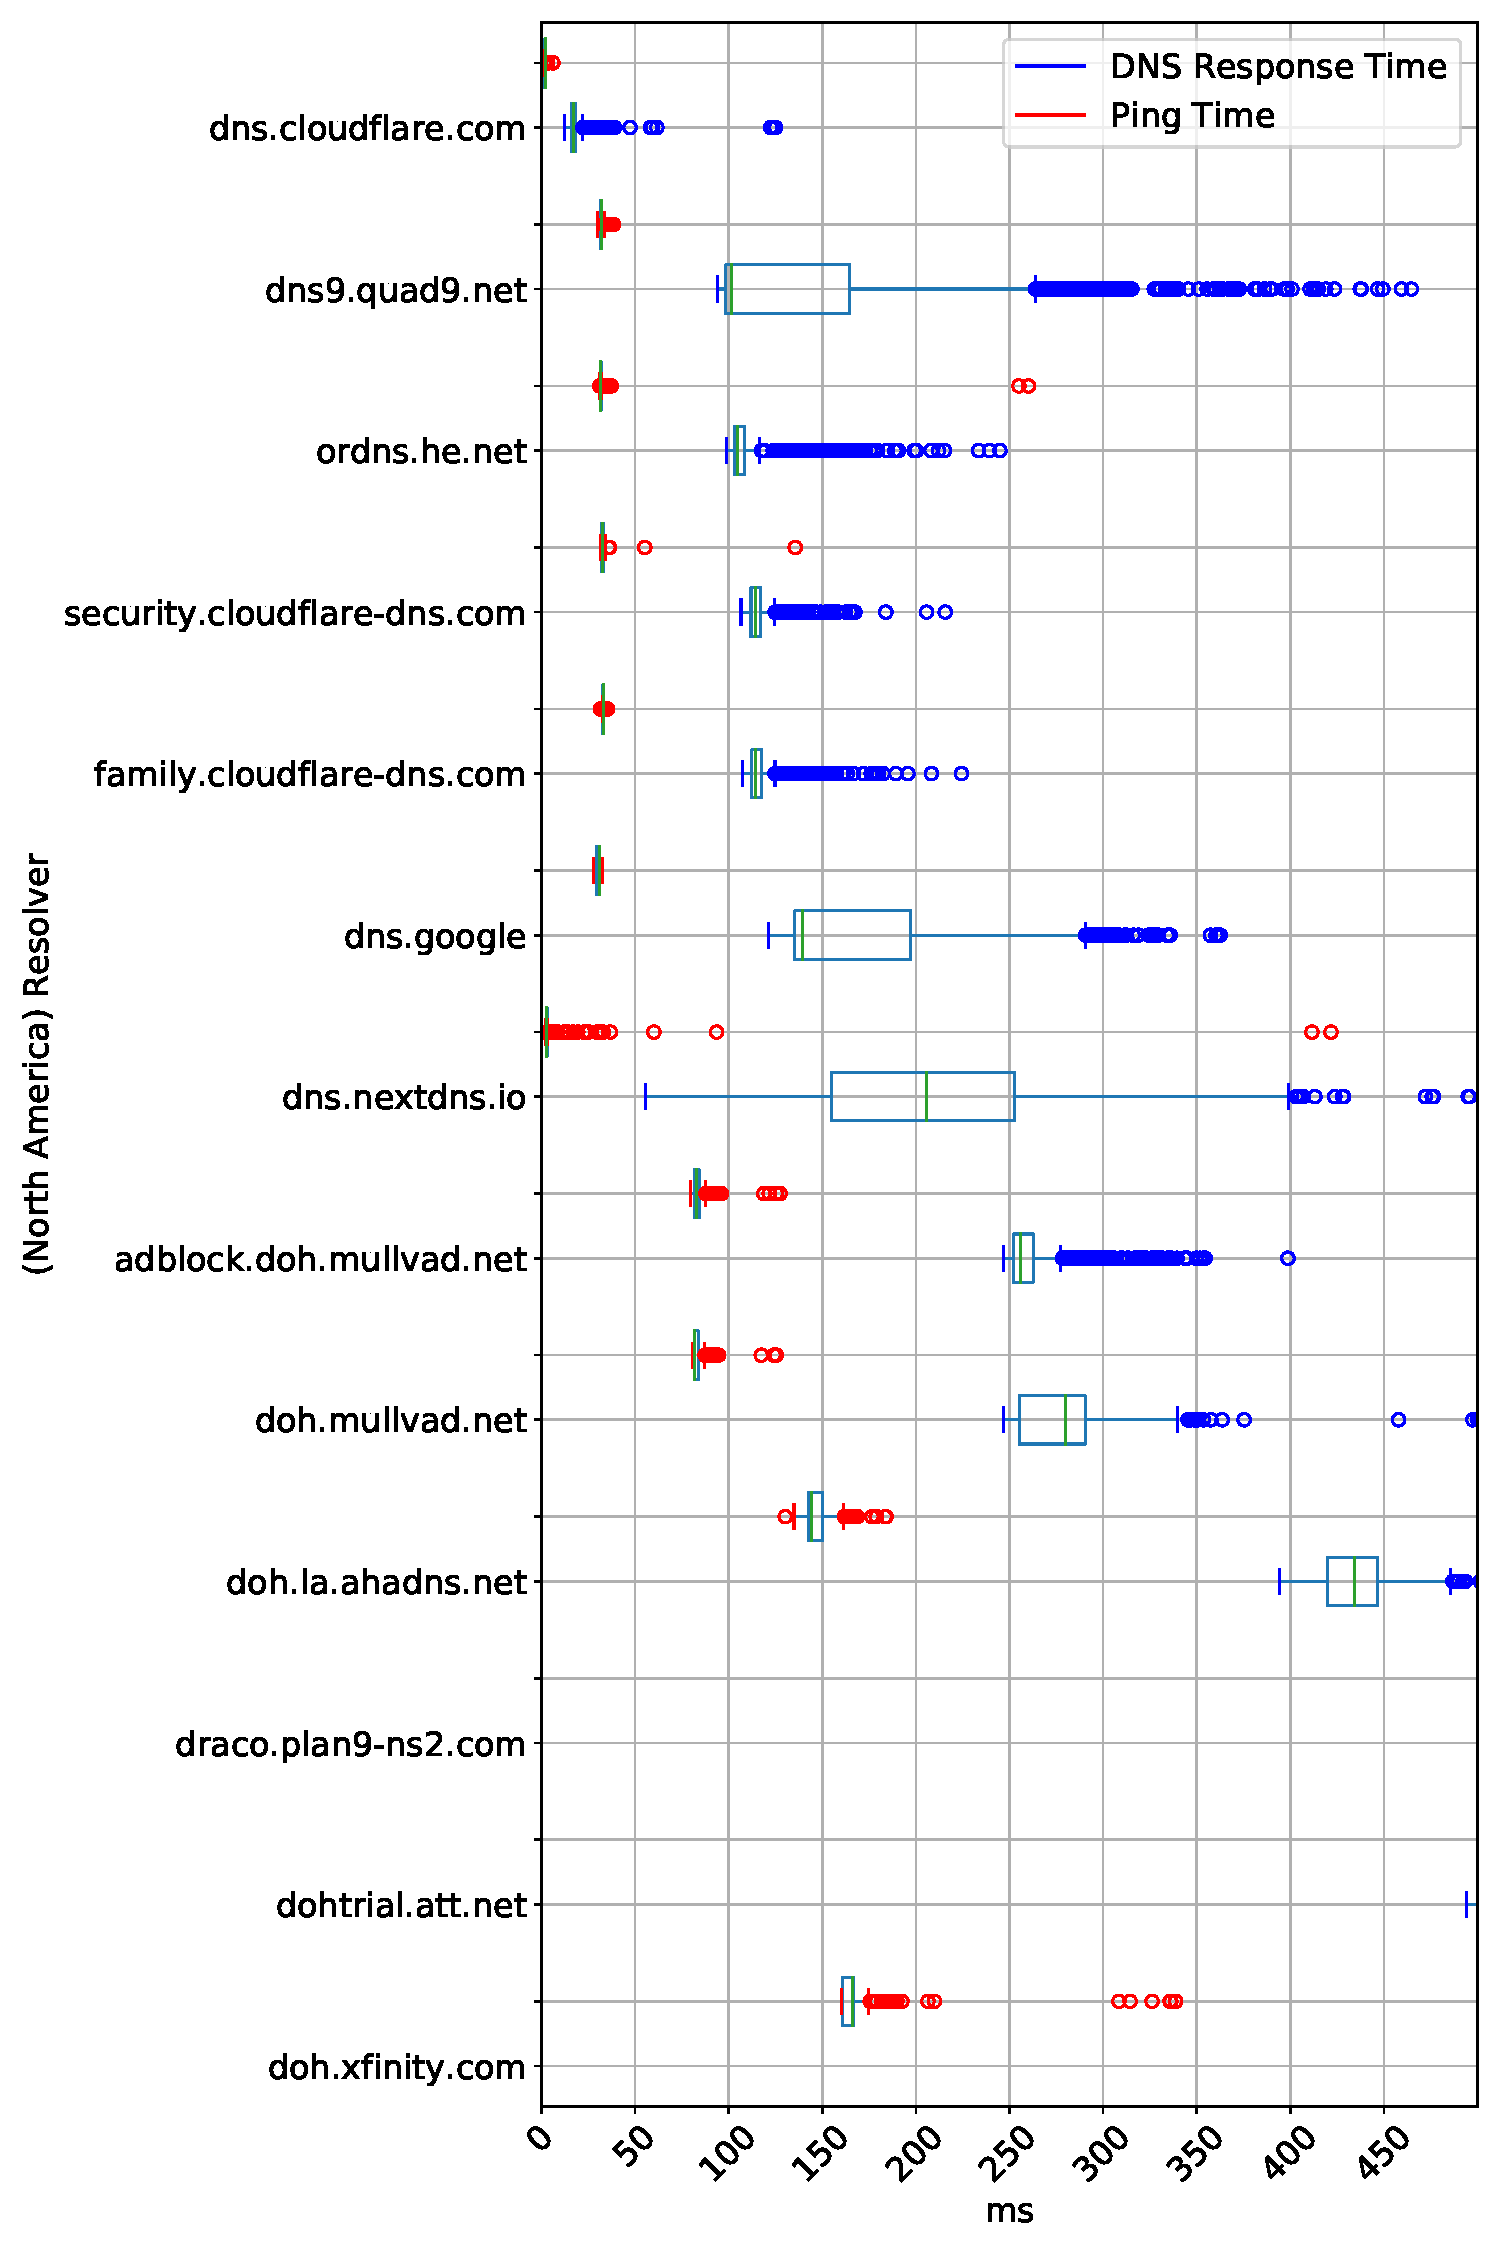
\includegraphics[width=0.32\linewidth]{figures/Seoul_North_America.pdf}}%
\hfill%
    \subfigure[Asia (Local).]{%
\label{fig:Seoul_Asia}%
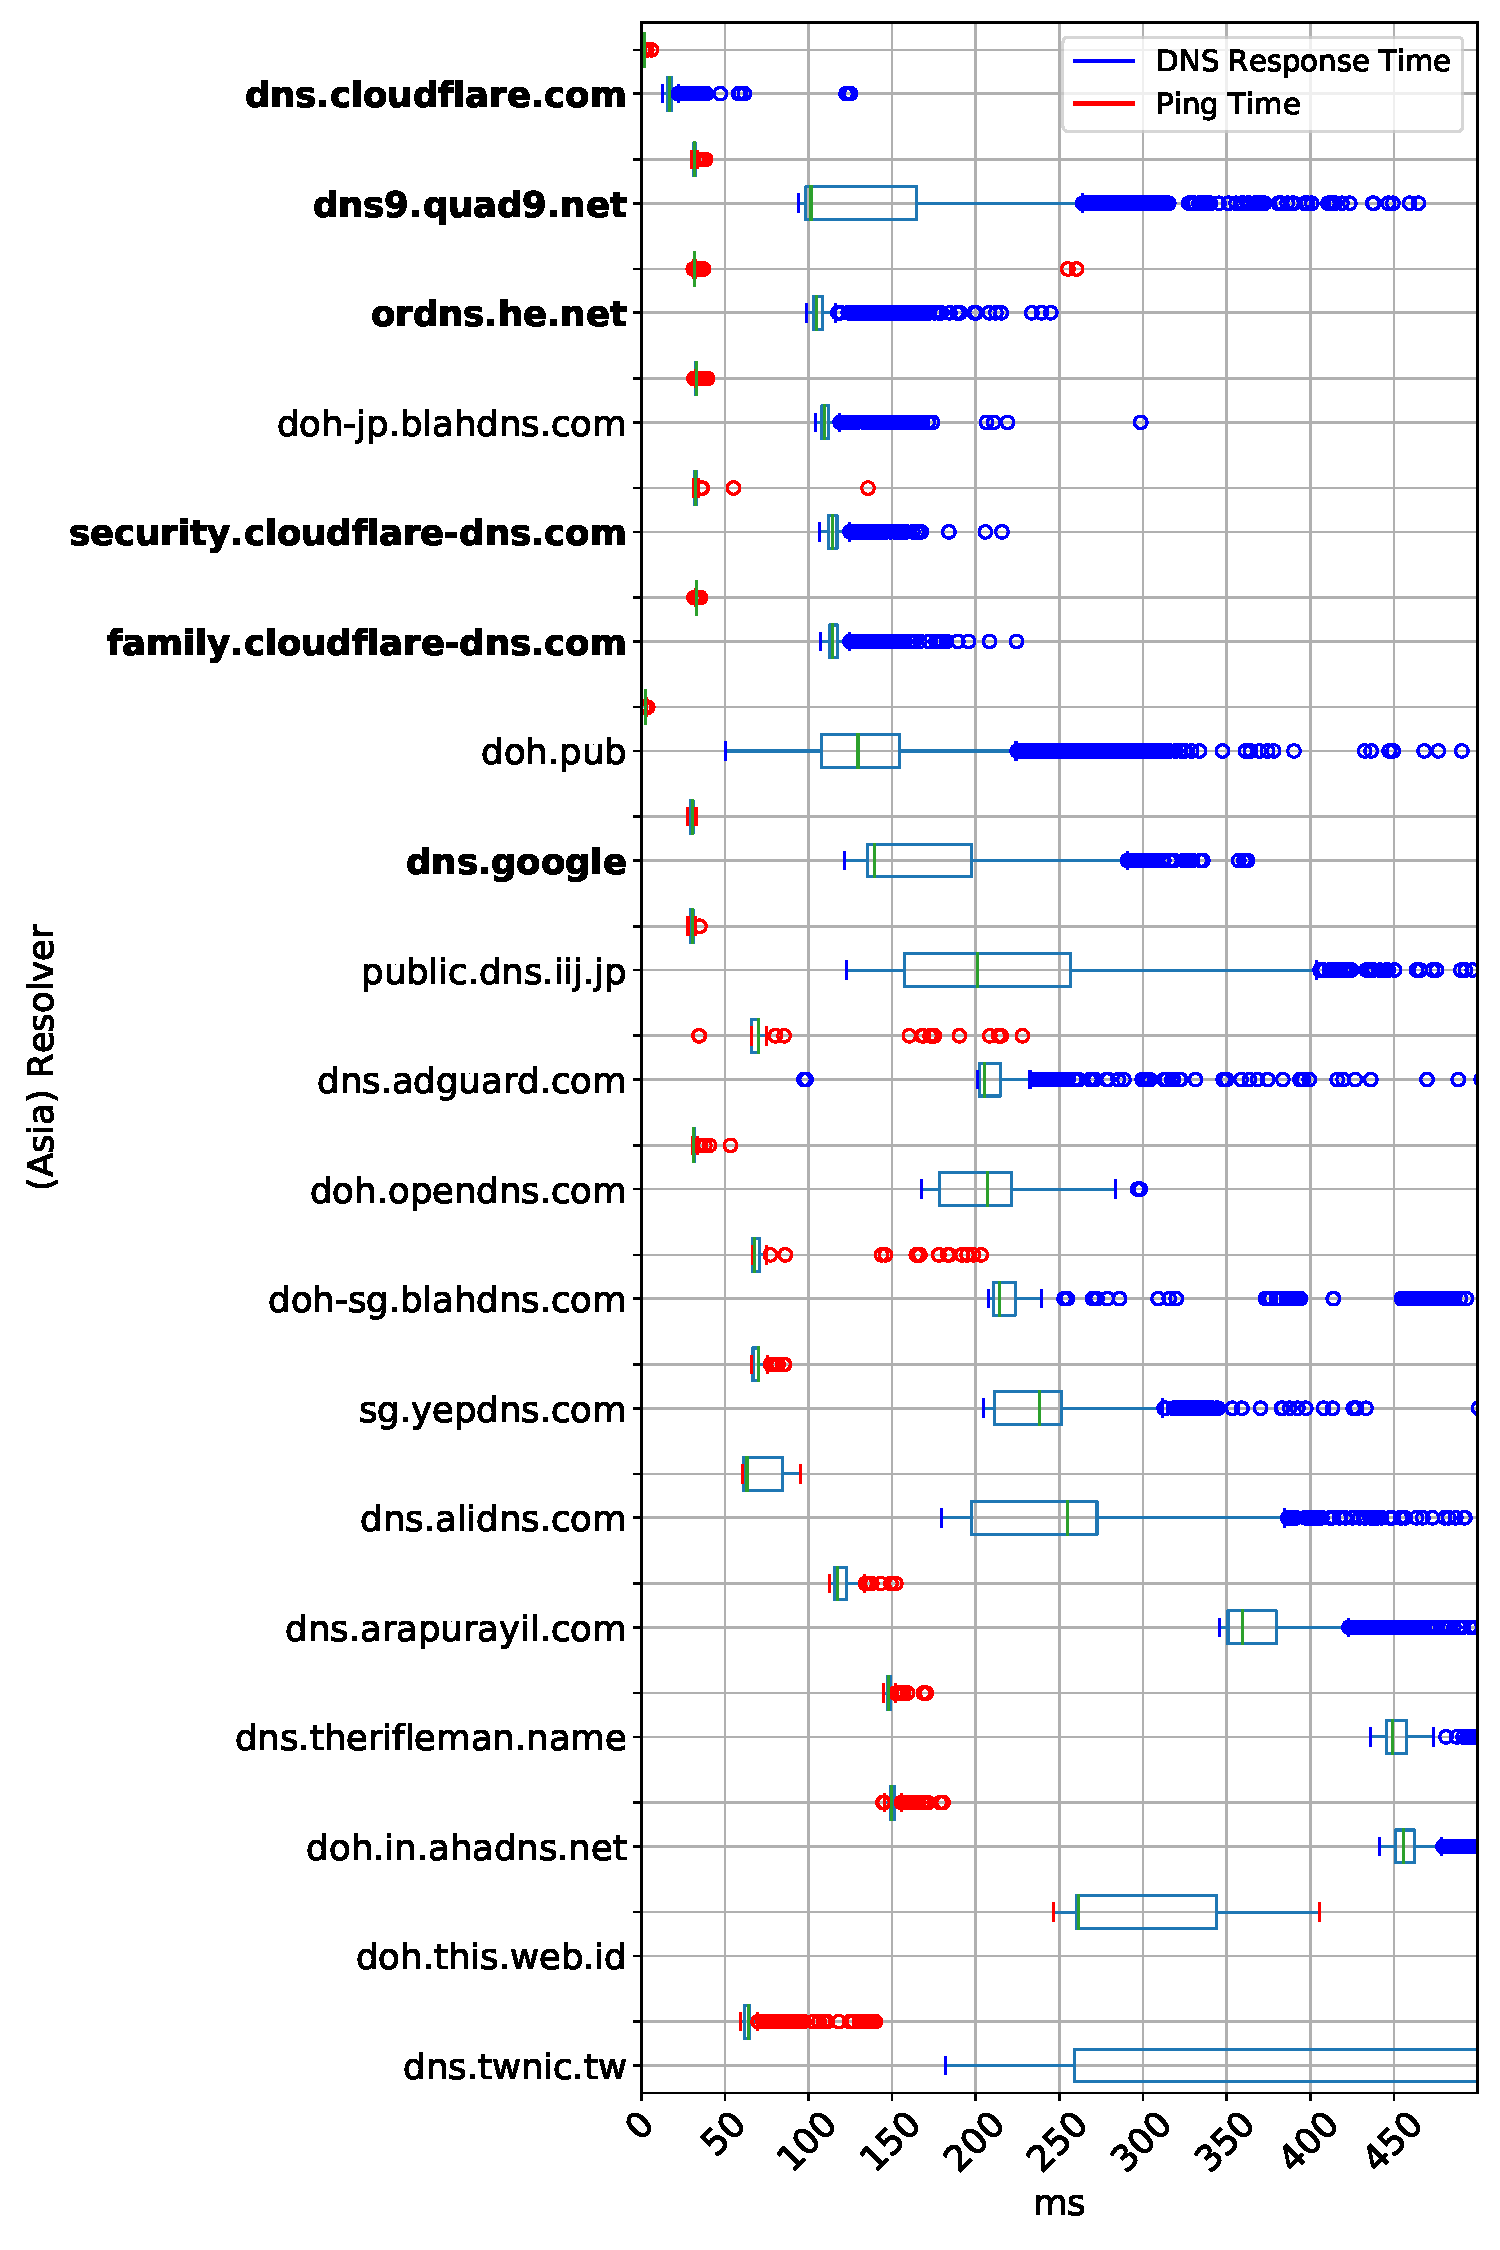
\includegraphics[width=0.32\linewidth]{figures/Seoul_Asia.pdf}}%
\hfill%
\subfigure[Europe.]{%
\label{fig:Seoul_Europe}%
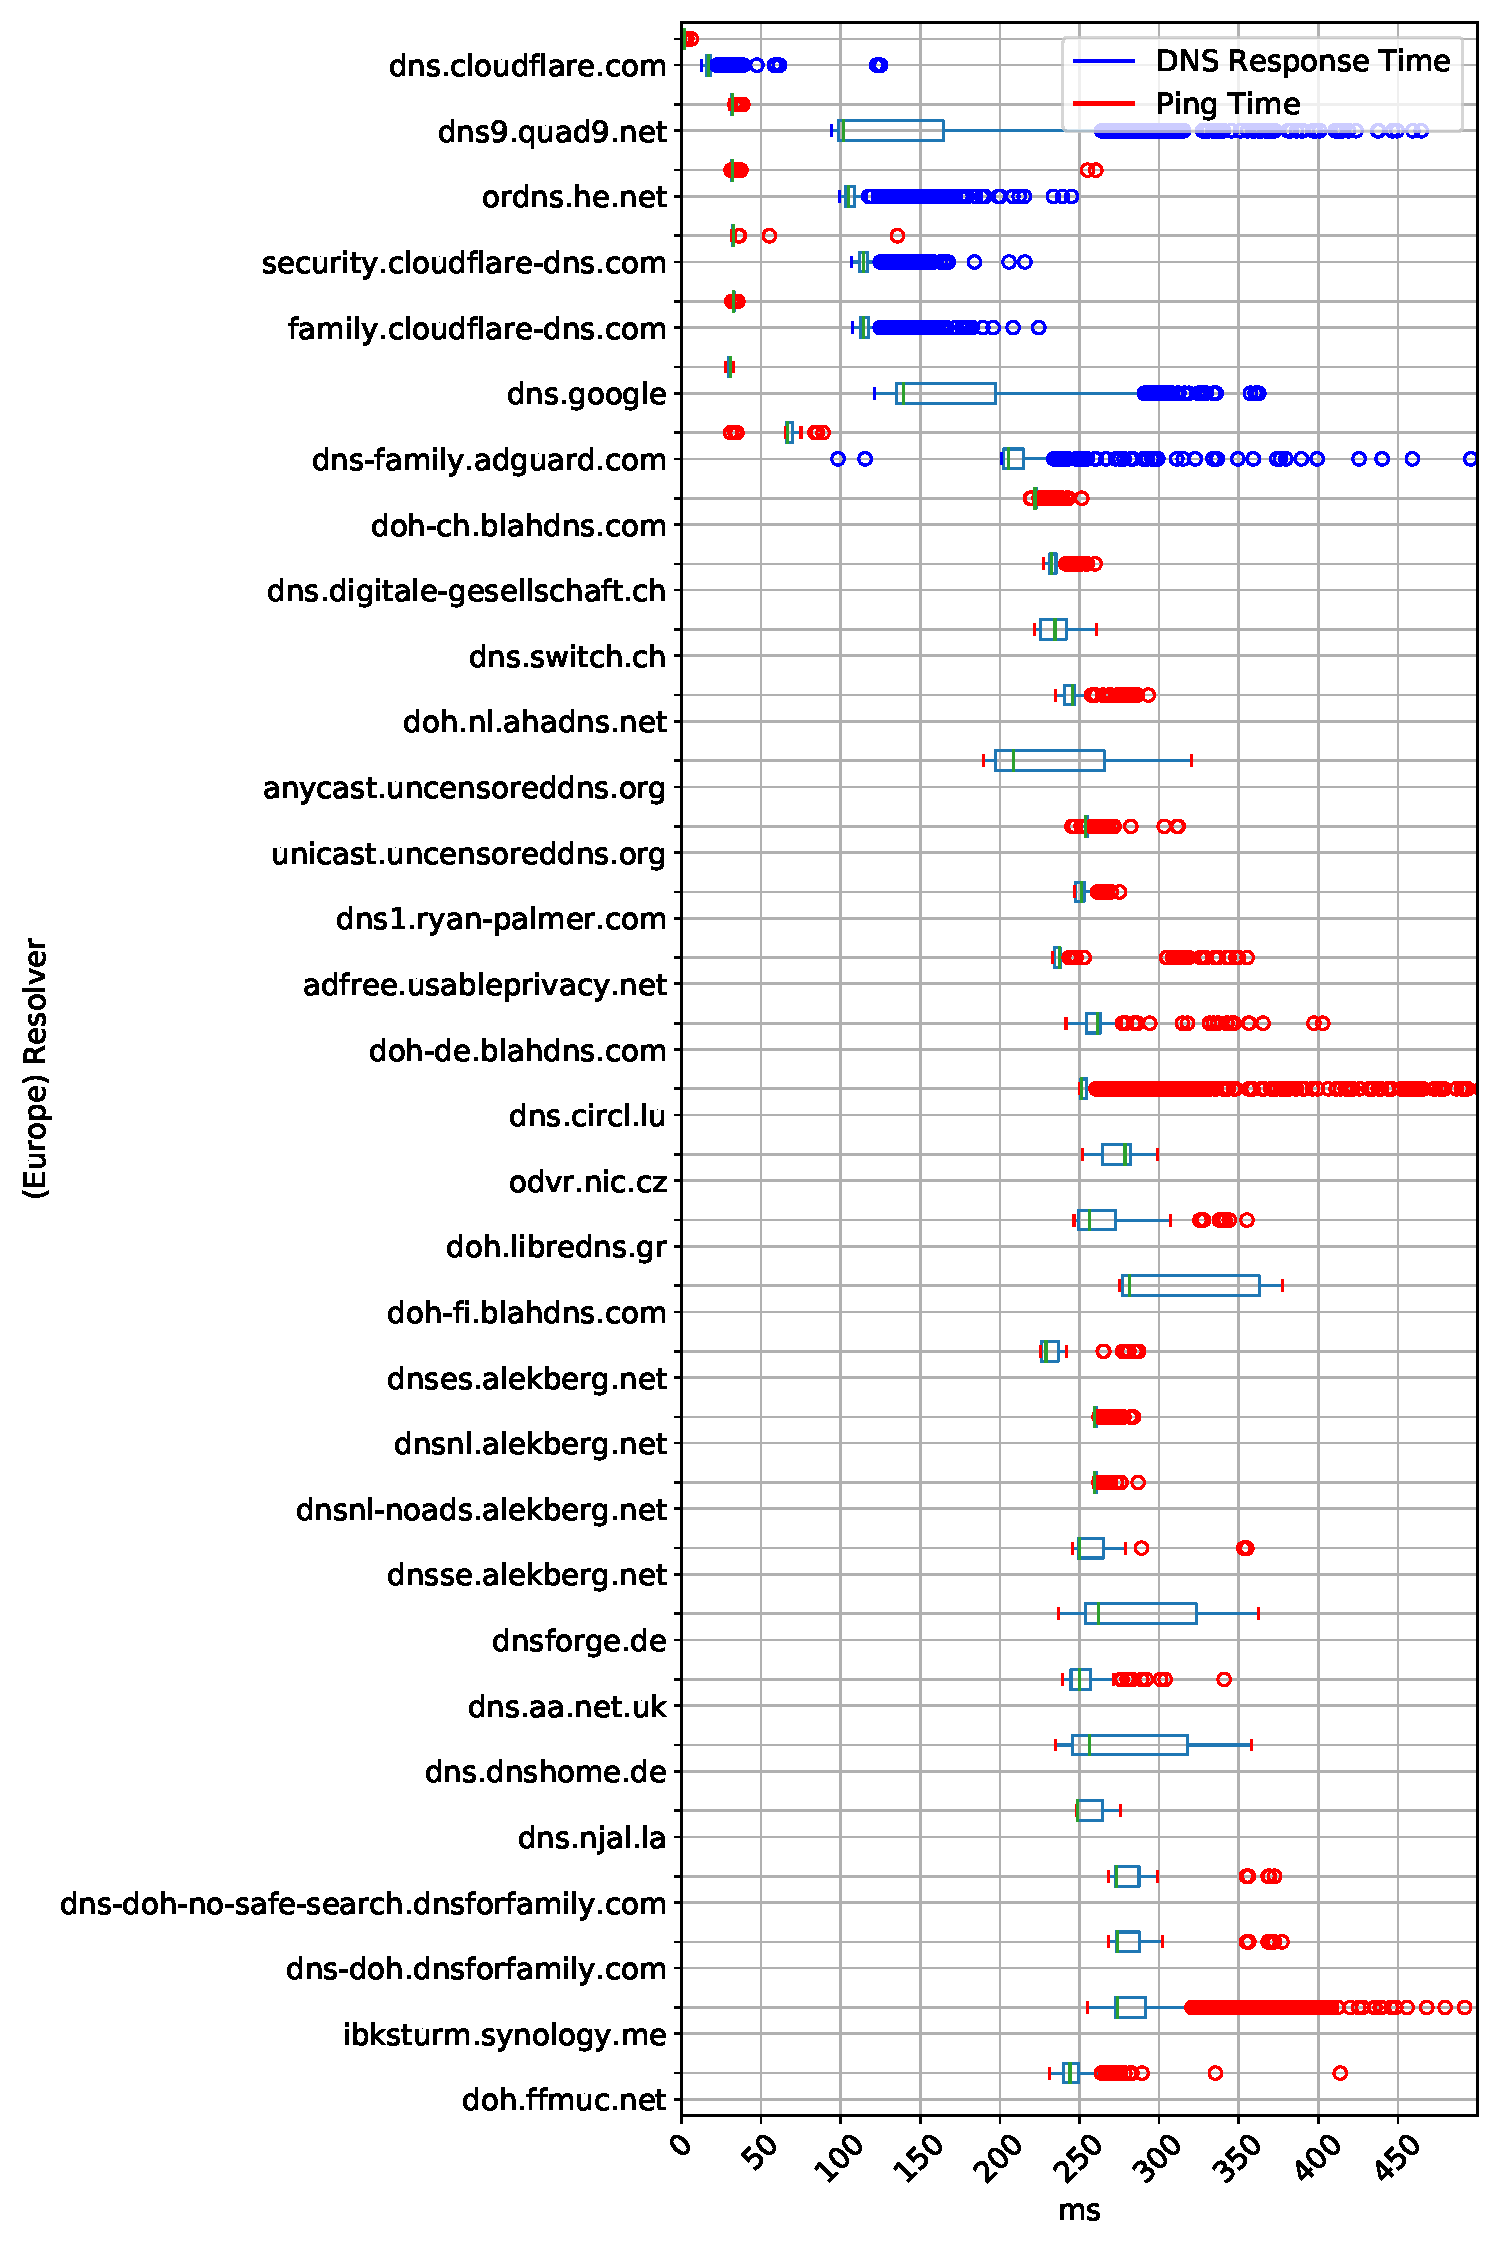
\includegraphics[width=0.32\linewidth]{figures/Seoul_Europe.pdf}}%
    \caption{The DNS response time and ICMP ping time distributions for
    encrypted DNS resolvers measured from a vantage point in Asia (Seoul, South
    Korea). Mainstream resolvers are shown in boldface across all three
    sub-figures.}
\label{fig:dns-asia}
\end{minipage}
\end{figure}


\if 0
\begin{table}[t!]
\centering
\begin{tabular}{ll}
\hline
\textbf{Location} & \textbf{Resolver}                                                                               \\ \hline
North America     & ordns.he.net                                                                                    \\ \hline
Asia              & \begin{tabular}[c]{@{}l@{}}ordns.he.net\\ doh-jp.blahdns.com\end{tabular}                       \\ \hline
Europe            & \begin{tabular}[c]{@{}l@{}}ordns.he.net\\ dns-family.adguard.com\\ doh.libredns.gr\end{tabular} \\ \hline
\end{tabular}
\caption{Non-mainstream resolvers that outperformed mainstream resolvers.}
\label{tab:outperformed_resolvers}
\end{table}
\fi




\begin{figure}[t!]
\hspace*{-1in}
\begin{minipage}{1.35\textwidth}
\centering
\subfigure[North America.]{%
\label{fig:Frankfurt_NA}%
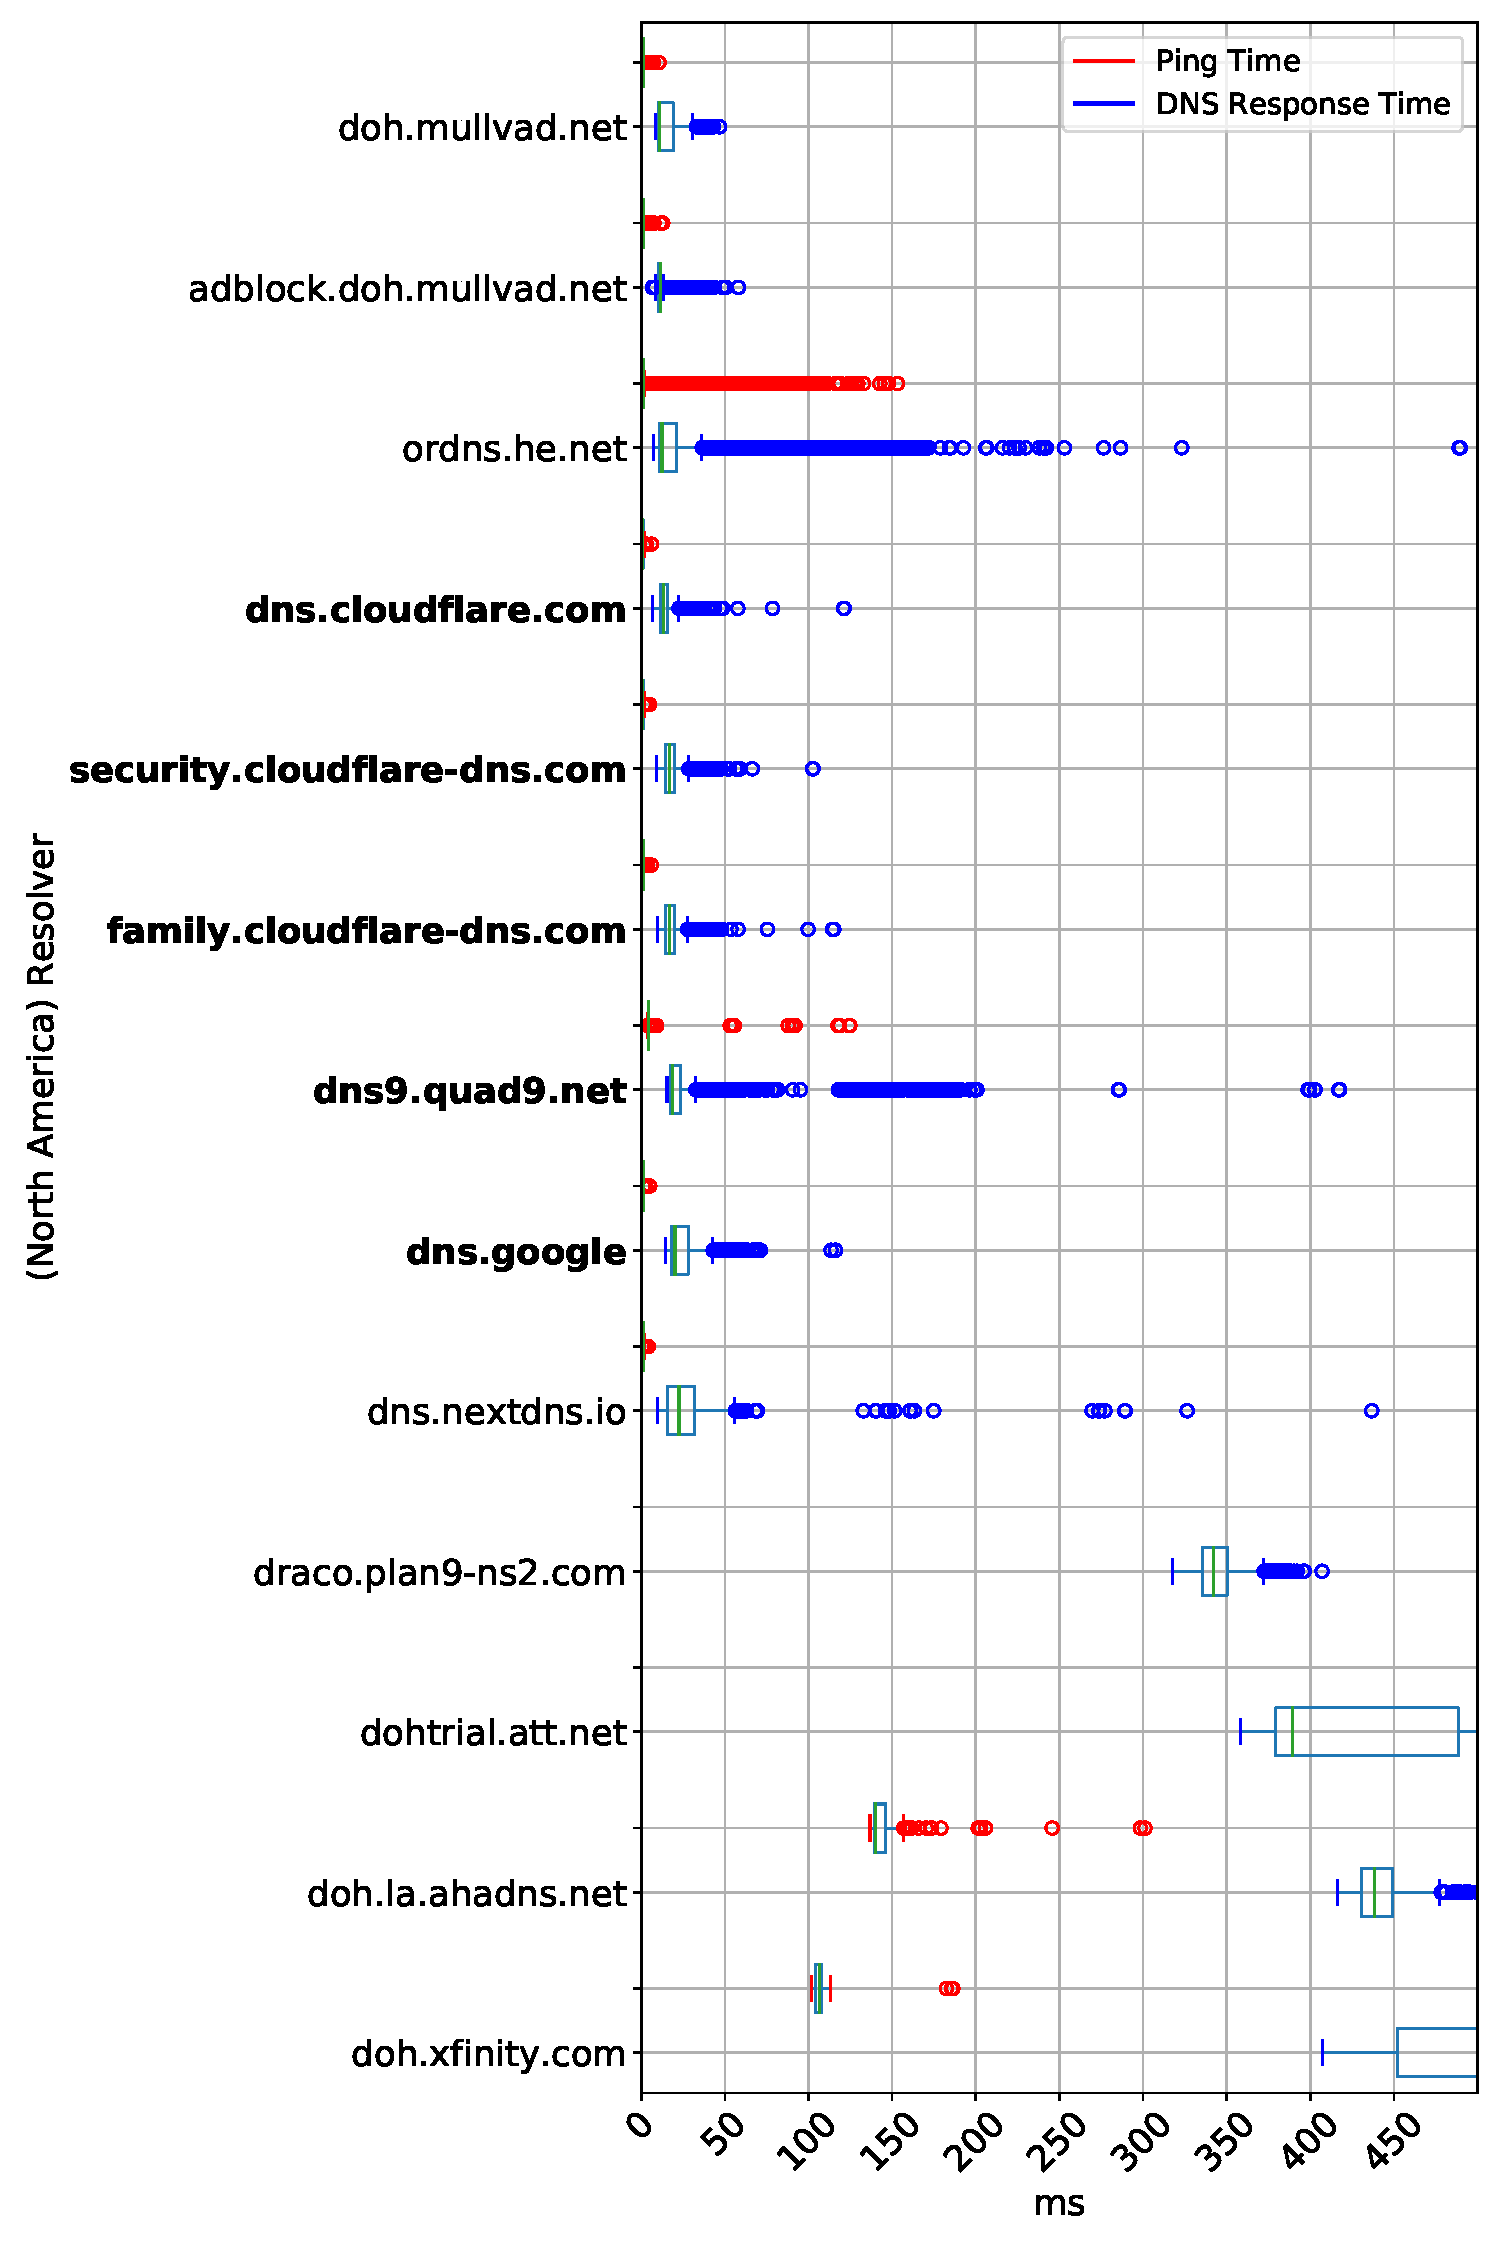
\includegraphics[width=0.32\linewidth]{figures/Frankfurt_North_America.pdf}}%
\hfill%
\subfigure[Asia. ]{%
\label{fig:Frankfurt_Asia}%
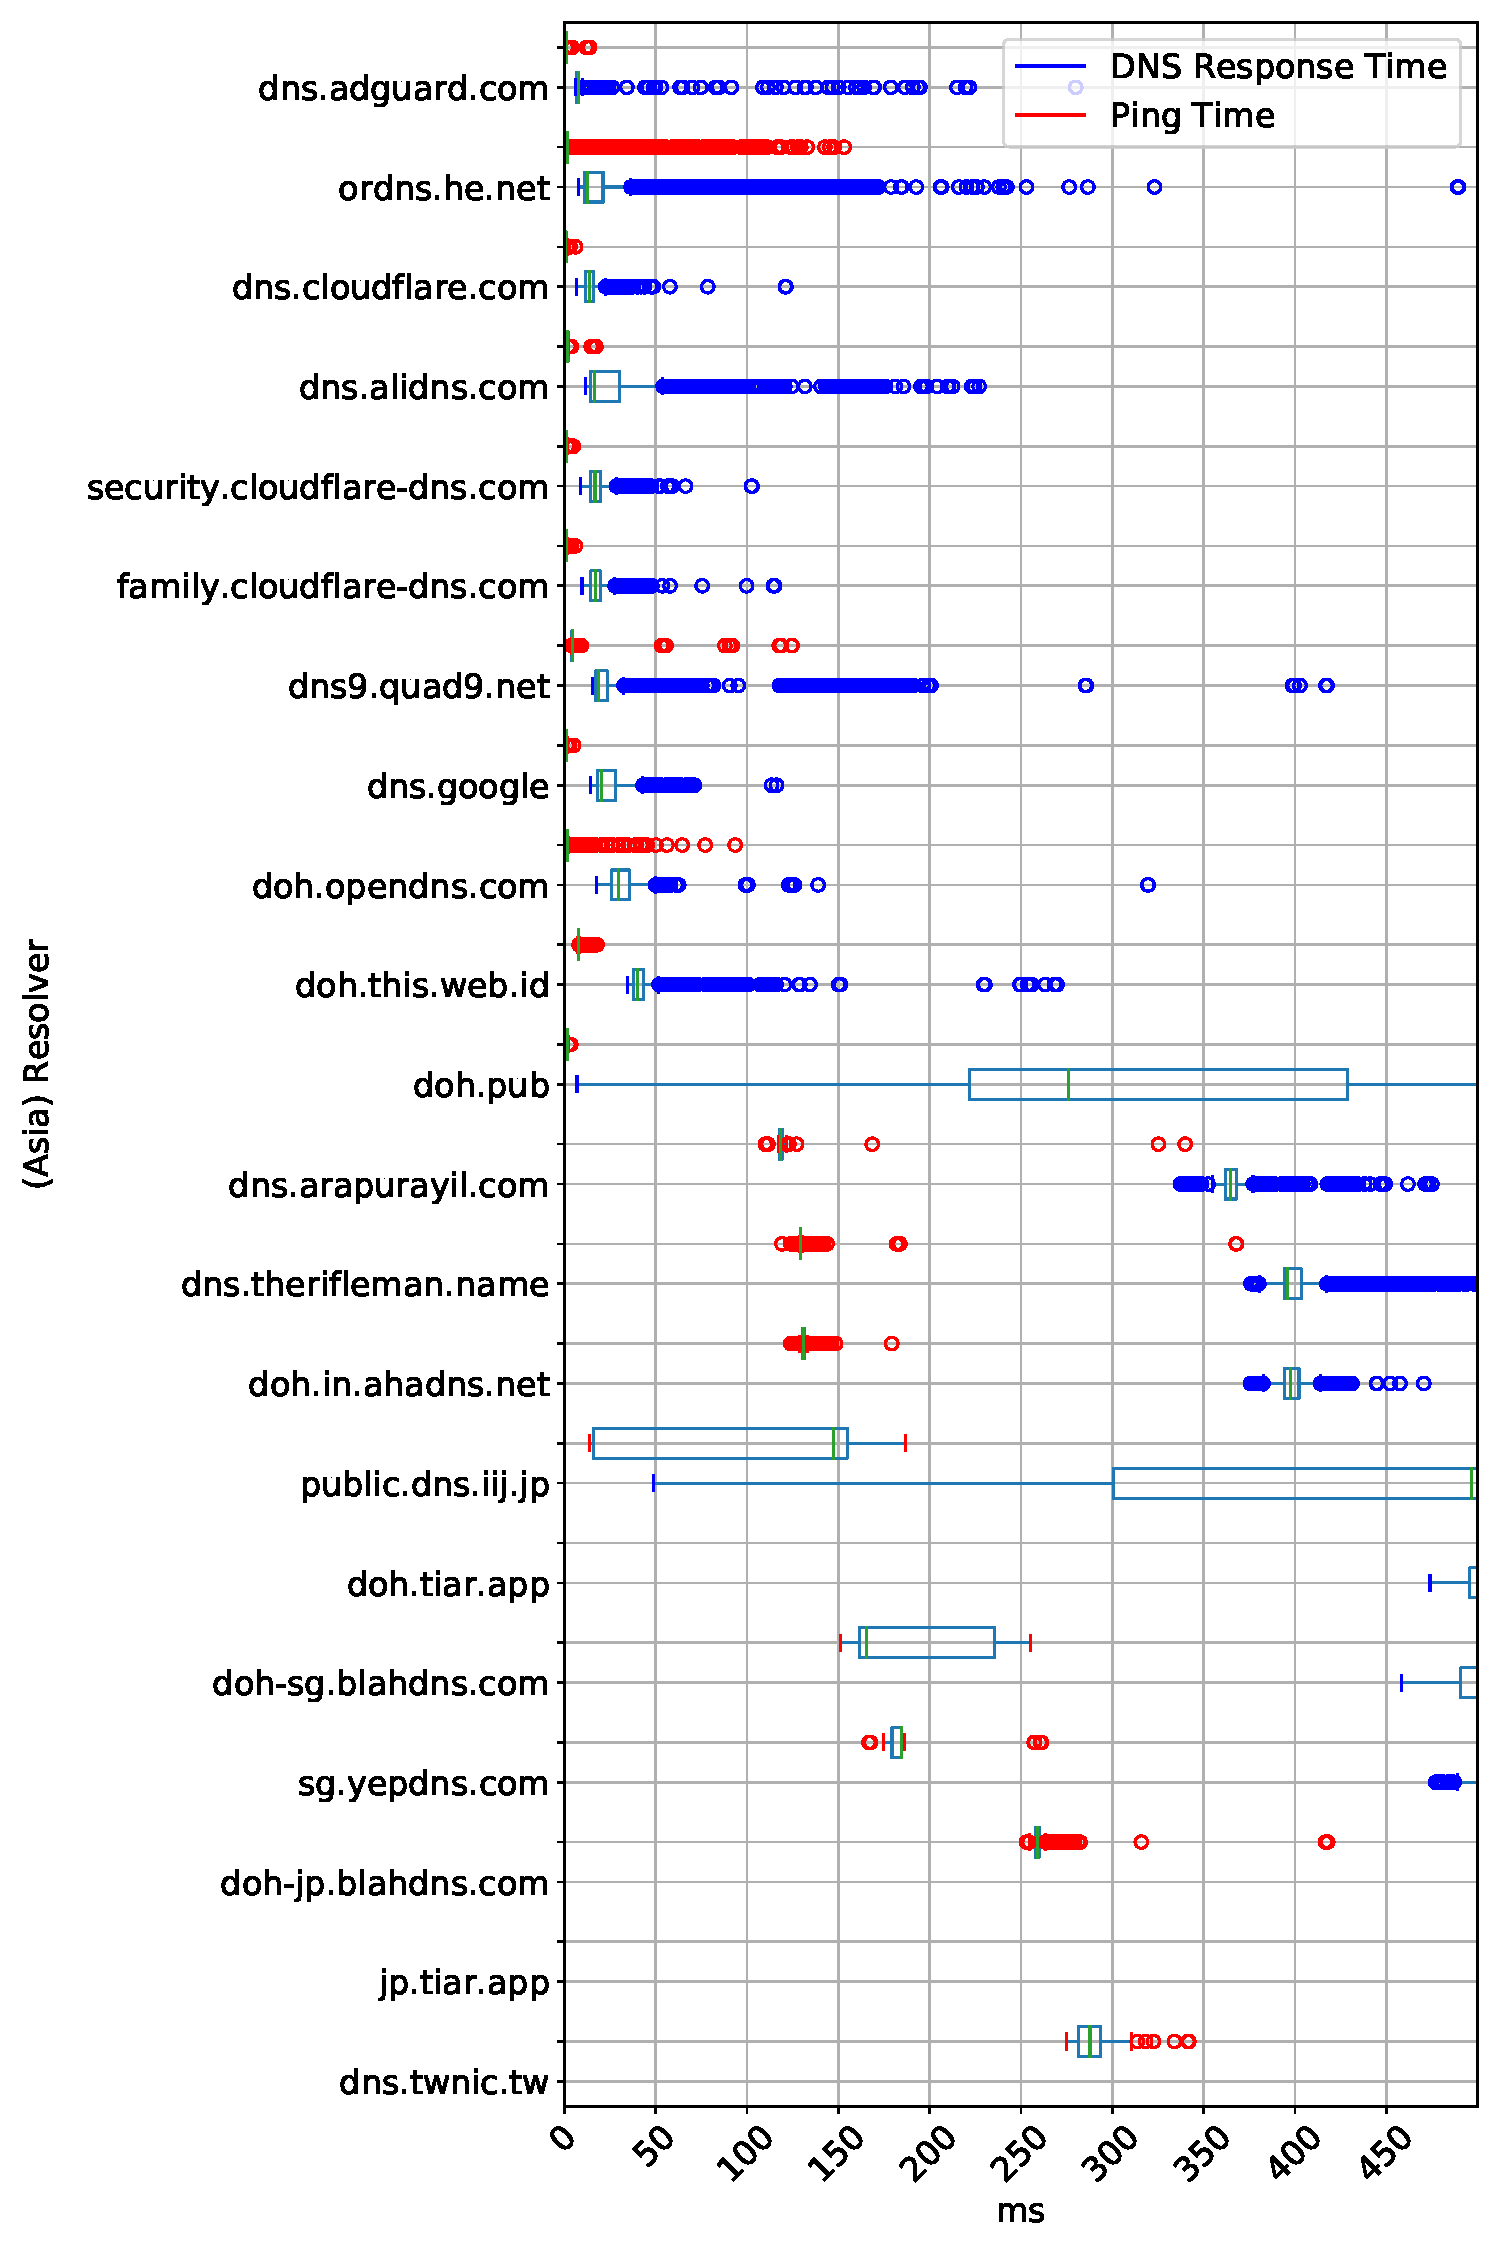
\includegraphics[width=0.32\linewidth]{figures/Frankfurt_Asia.pdf}}%
\hfill%
\subfigure[Europe (Local).]{%
\label{fig:Frankfurt_Europe}%
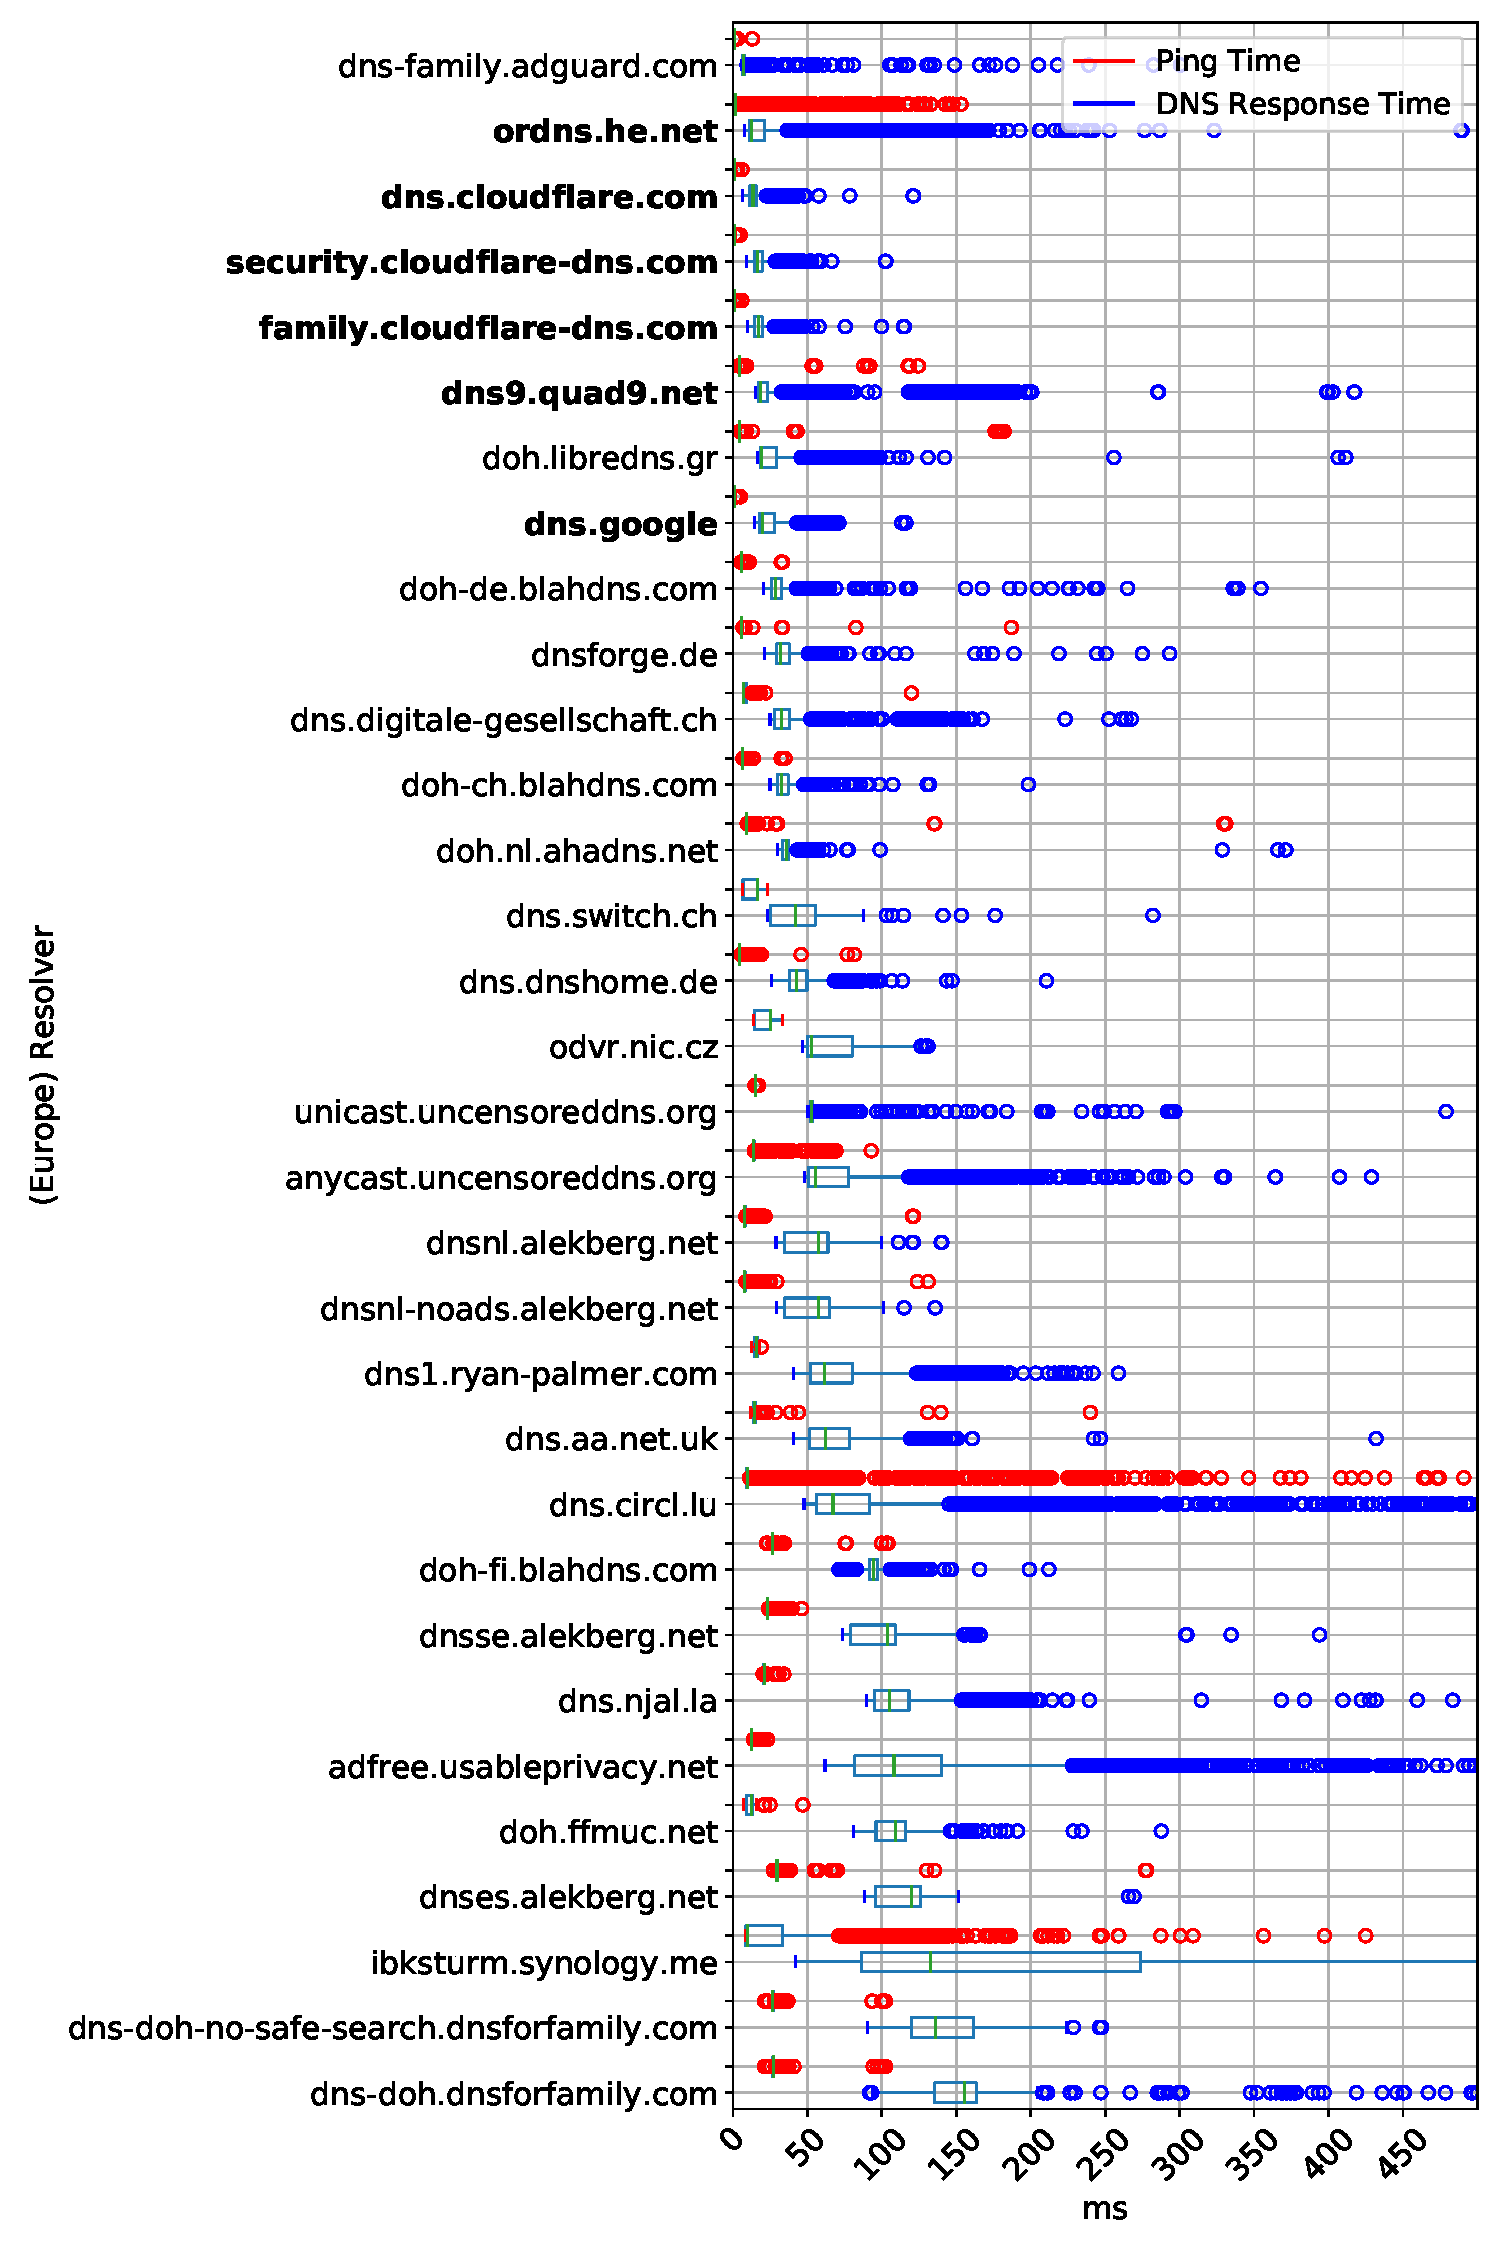
\includegraphics[width=0.32\linewidth]{figures/Frankfurt_Europe.pdf}}%
    \caption{The DNS response time and ICMP ping time distributions for
    encrypted DNS resolvers measured from a vantage point in Europe (Germany). Mainstream resolvers are shown in boldface across all three
    sub-figures.}
\label{fig:dns-europe}
\end{minipage}
\end{figure}

\begin{table}[t!]
\hspace*{-0.75in}
\begin{minipage}{1.25\linewidth}
\parbox{0.45\linewidth}{
\begin{scriptsize}
\centering
\begin{tabular}{l|rr}
\toprule
    \textbf{Resolver} & \multicolumn{2}{c}{\textbf{Vantage Point}} \\
                  & \textrm{Seoul (ms)}         & \textrm{Frankfurt (ms)} \\
\midrule
dns.twnic.tw                                & 31606.61 & 32319.90                            \\
doh-jp.blahdns.com                          & 109.62                                           & 773.47                              \\
sg.yepdns.com                               & 238.01                                           & 548.67                              \\
public.dns.iij.jp                           & 200.82                                           & 496.74                             \\
doh-sg.blahdns                              & 214.44                                           & 534.51                               \\
\bottomrule
\end{tabular}
\end{scriptsize}
    \caption{Median DNS response times for non-mainstream resolvers (Asia).}
\label{tab:UnconvAsia}
}\hfill
%\end{table}
%\begin{table}[t!]
\centering
\parbox{0.45\linewidth}{
\begin{scriptsize}
\begin{tabular}{l|rr}
\toprule
\textbf{Resolver} & \multicolumn{2}{c}{\textbf{Vantage Point}} \\
                  & \textrm{Frankfurt (ms)}     & \textrm{Seoul (ms)} \\
\midrule
doh.ffmuc.net                               & 108.92 & 1309.88                         \\
ibksturm.synology.me                        & 132.66 & 1254.47                         \\
dns-doh-no-safe-search.dnsforfamily         & 135.88 & 1159.70                         \\
dnsforge.de                                 & 31.86 & 1043.03                         \\
dns-doh.dnsforfamily                        & 155.81 & 1162.27                         \\
\bottomrule
\end{tabular}
\end{scriptsize}
    \caption{Median DNS response times for non-mainstream resolvers (Europe).}
\label{tab:UnconvEur}
}
\end{minipage}
\end{table}


To better understand the extent to which certain encrypted DNS resolvers
perform well for clients in some regions but not others, we identified
resolvers that exhibited low DNS response times in for clients in one region
but not another. 
Tables~\ref{tab:UnconvAsia} and~\ref{tab:UnconvEur} show 
the five encrypted DNS resolvers for Europe and Asia that exhibit the 
largest differences in median DNS response times when
queried from a remote vantage point (queries of resolvers in Asia from Europe,
and of resolvers of Europe from Asia, respectively). In both cases, 
Table~\ref{tab:UnconvAsia} shows that non-mainstream resolvers located
in Asia perform better from the vantage point in Seoul than the one in
Frankfurt.  Similarly, as expected, Table~\ref{tab:UnconvEur} shows that the
median response times of non-mainstream resolvers in Europe are much lower when
measured from Frankfurt than the response times of those same resolvers
measured from Seoul.

\subsection{Does Latency to Resolver Correlate with Performance?}

Figure~\ref{fig:ping_qrt_scatters} compares median ICMP ping latencies to median 
query response times for each resolver.
Higher network latency naturally translates to higher DNS response
times (as encrypted DNS queries do require several network round trips):
absent connection re-use, a DoH lookup will require at least three network
round trips: one for the TCP three-way handshake, one for the TLS handshake
(piggybacked on the third part of the three-way handshake), and one for the
DNS query and response. {\tt libcurl} uses TLS 1.3 when available on the
server, and otherwise falls back to an older version (e.g., TLS 1.2), which requires an additional
network round trip.
It also attempts to use HTTP/2, falling back to an older version when necessary.
Thus, we can expect that ``normal'' DoH lookup times would
be about 3--4 times the network latency.

\begin{figure*}[t]
    \hspace*{-0.75in}
    \begin{minipage}{1.35\linewidth}
    \subfigure[Ohio (Local).]{%
        \label{fig:Ohio_ping_qrt_scatter}
        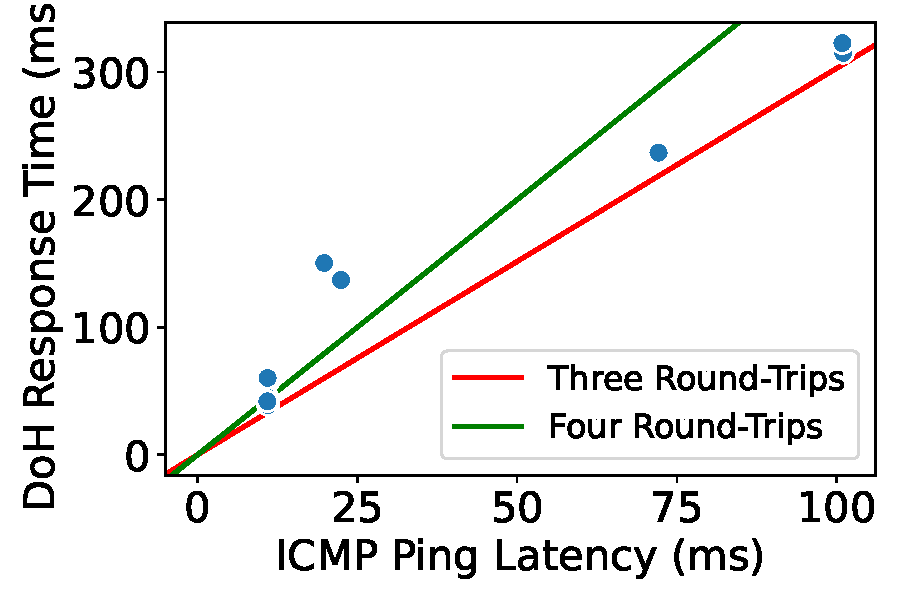
\includegraphics[width=0.3\linewidth]{figures/Ohio_ping_qrt_scatter.pdf}
    }
    \hfill
    \subfigure[Seoul (Local).]{%
        \label{fig:Seoul_ping_qrt_scatter}
        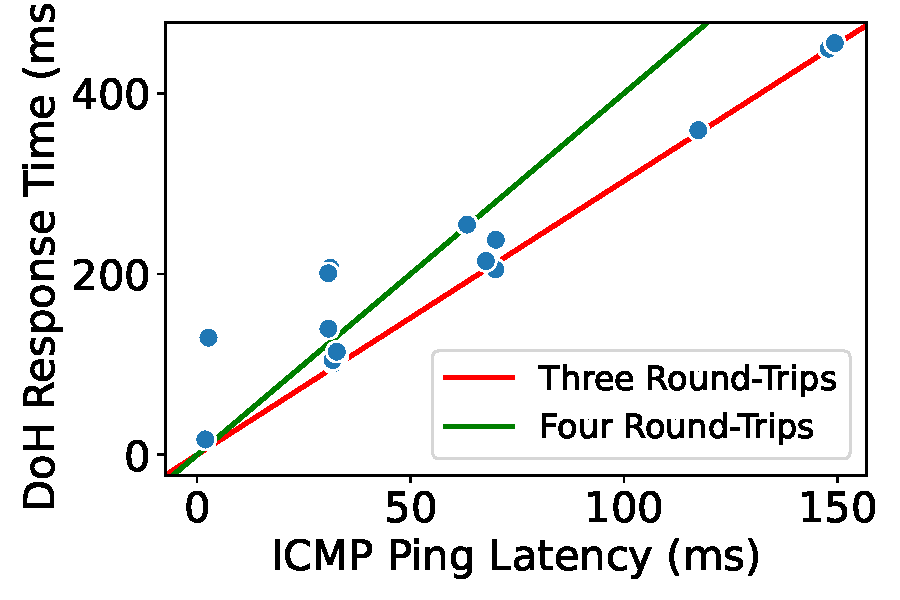
\includegraphics[width=0.3\linewidth]{figures/Seoul_ping_qrt_scatter.pdf}
    }
    \hfill
    \subfigure[Frankfurt (Local).]{%
        \label{fig:Frankfurt_ping_qrt_scatter}
        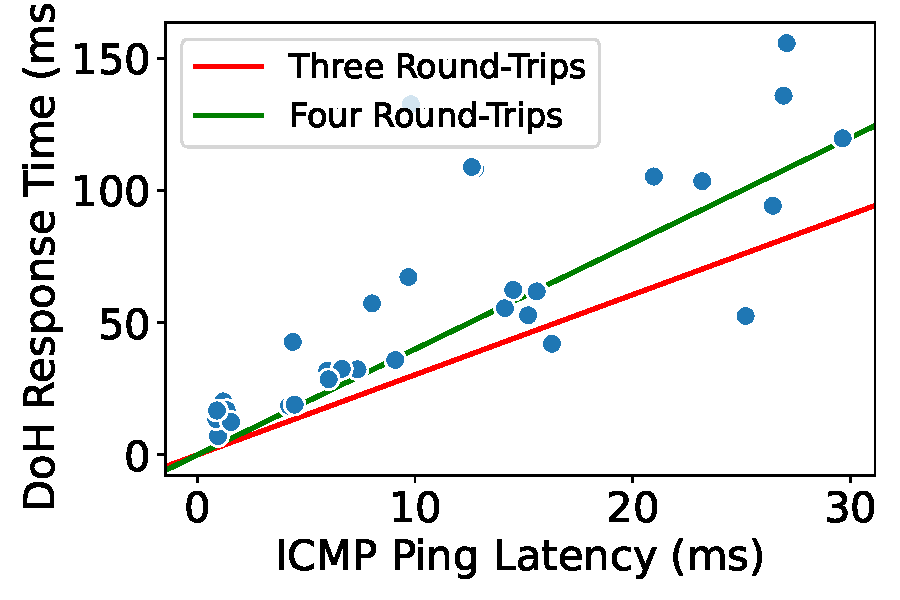
\includegraphics[width=0.3\linewidth]{figures/Frankfurt_ping_qrt_scatter.pdf}
    }
    \caption{Median DoH query response times vs. median round-trip network
    latency for each local DoH resolver, from each vantage point.}
    \label{fig:ping_qrt_scatters}
    \end{minipage}
\end{figure*}



In some cases, certain resolvers performed worse than might
be expected as a result of the latency from the vantage point to the
resolvers. 
%For example, although the median round-trip latency to
%\texttt{doh.in.ahadns.net} from our Seoul vantage point was 149~ms, the
%median query response time was~456 ms. 
For example, from North America, we
observed a median query response time of 872 ms to \texttt{doh.xfinity.com} 
despite a network round-trip latency of merely 166~ms.
Many non-mainstream resolvers in Europe and Asia exhibit encrypted DNS
response times that are more than 4x the round-trip network latency.
These discrepancies between network latency and DNS response times may be due 
to a number of factors, including both caching and server load.

From Frankfurt, we observed two resolvers with median DoH query response
times that are less than 3--4 times the median network latency to these resolvers:
\texttt{dns.switch.ch} and \texttt{odvr.nic.cz}.
We hypothesize that this could be attributed to anomalous ICMP ping data and
network optimizations that enable DoH queries to be completed in fewer
round-trips.
Two resolvers---\texttt{doh.this.web.id} and
\texttt{dns.twnic.tw}---are not shown in Figure~\ref{fig:Seoul_ping_qrt_scatter}
because their median query response times are greater than 1,000 ms.
For reference, the next slowest resolver from Seoul has a median query response
time of 456~ms.

\if 0
\begin{figure}[t!]
\hspace*{-0.75in}
\begin{minipage}{1.25\textwidth}
\centering
\subfigure[North American resolvers measured from Ohio, USA]{%
\label{fig:Local_Ohio_NA}%
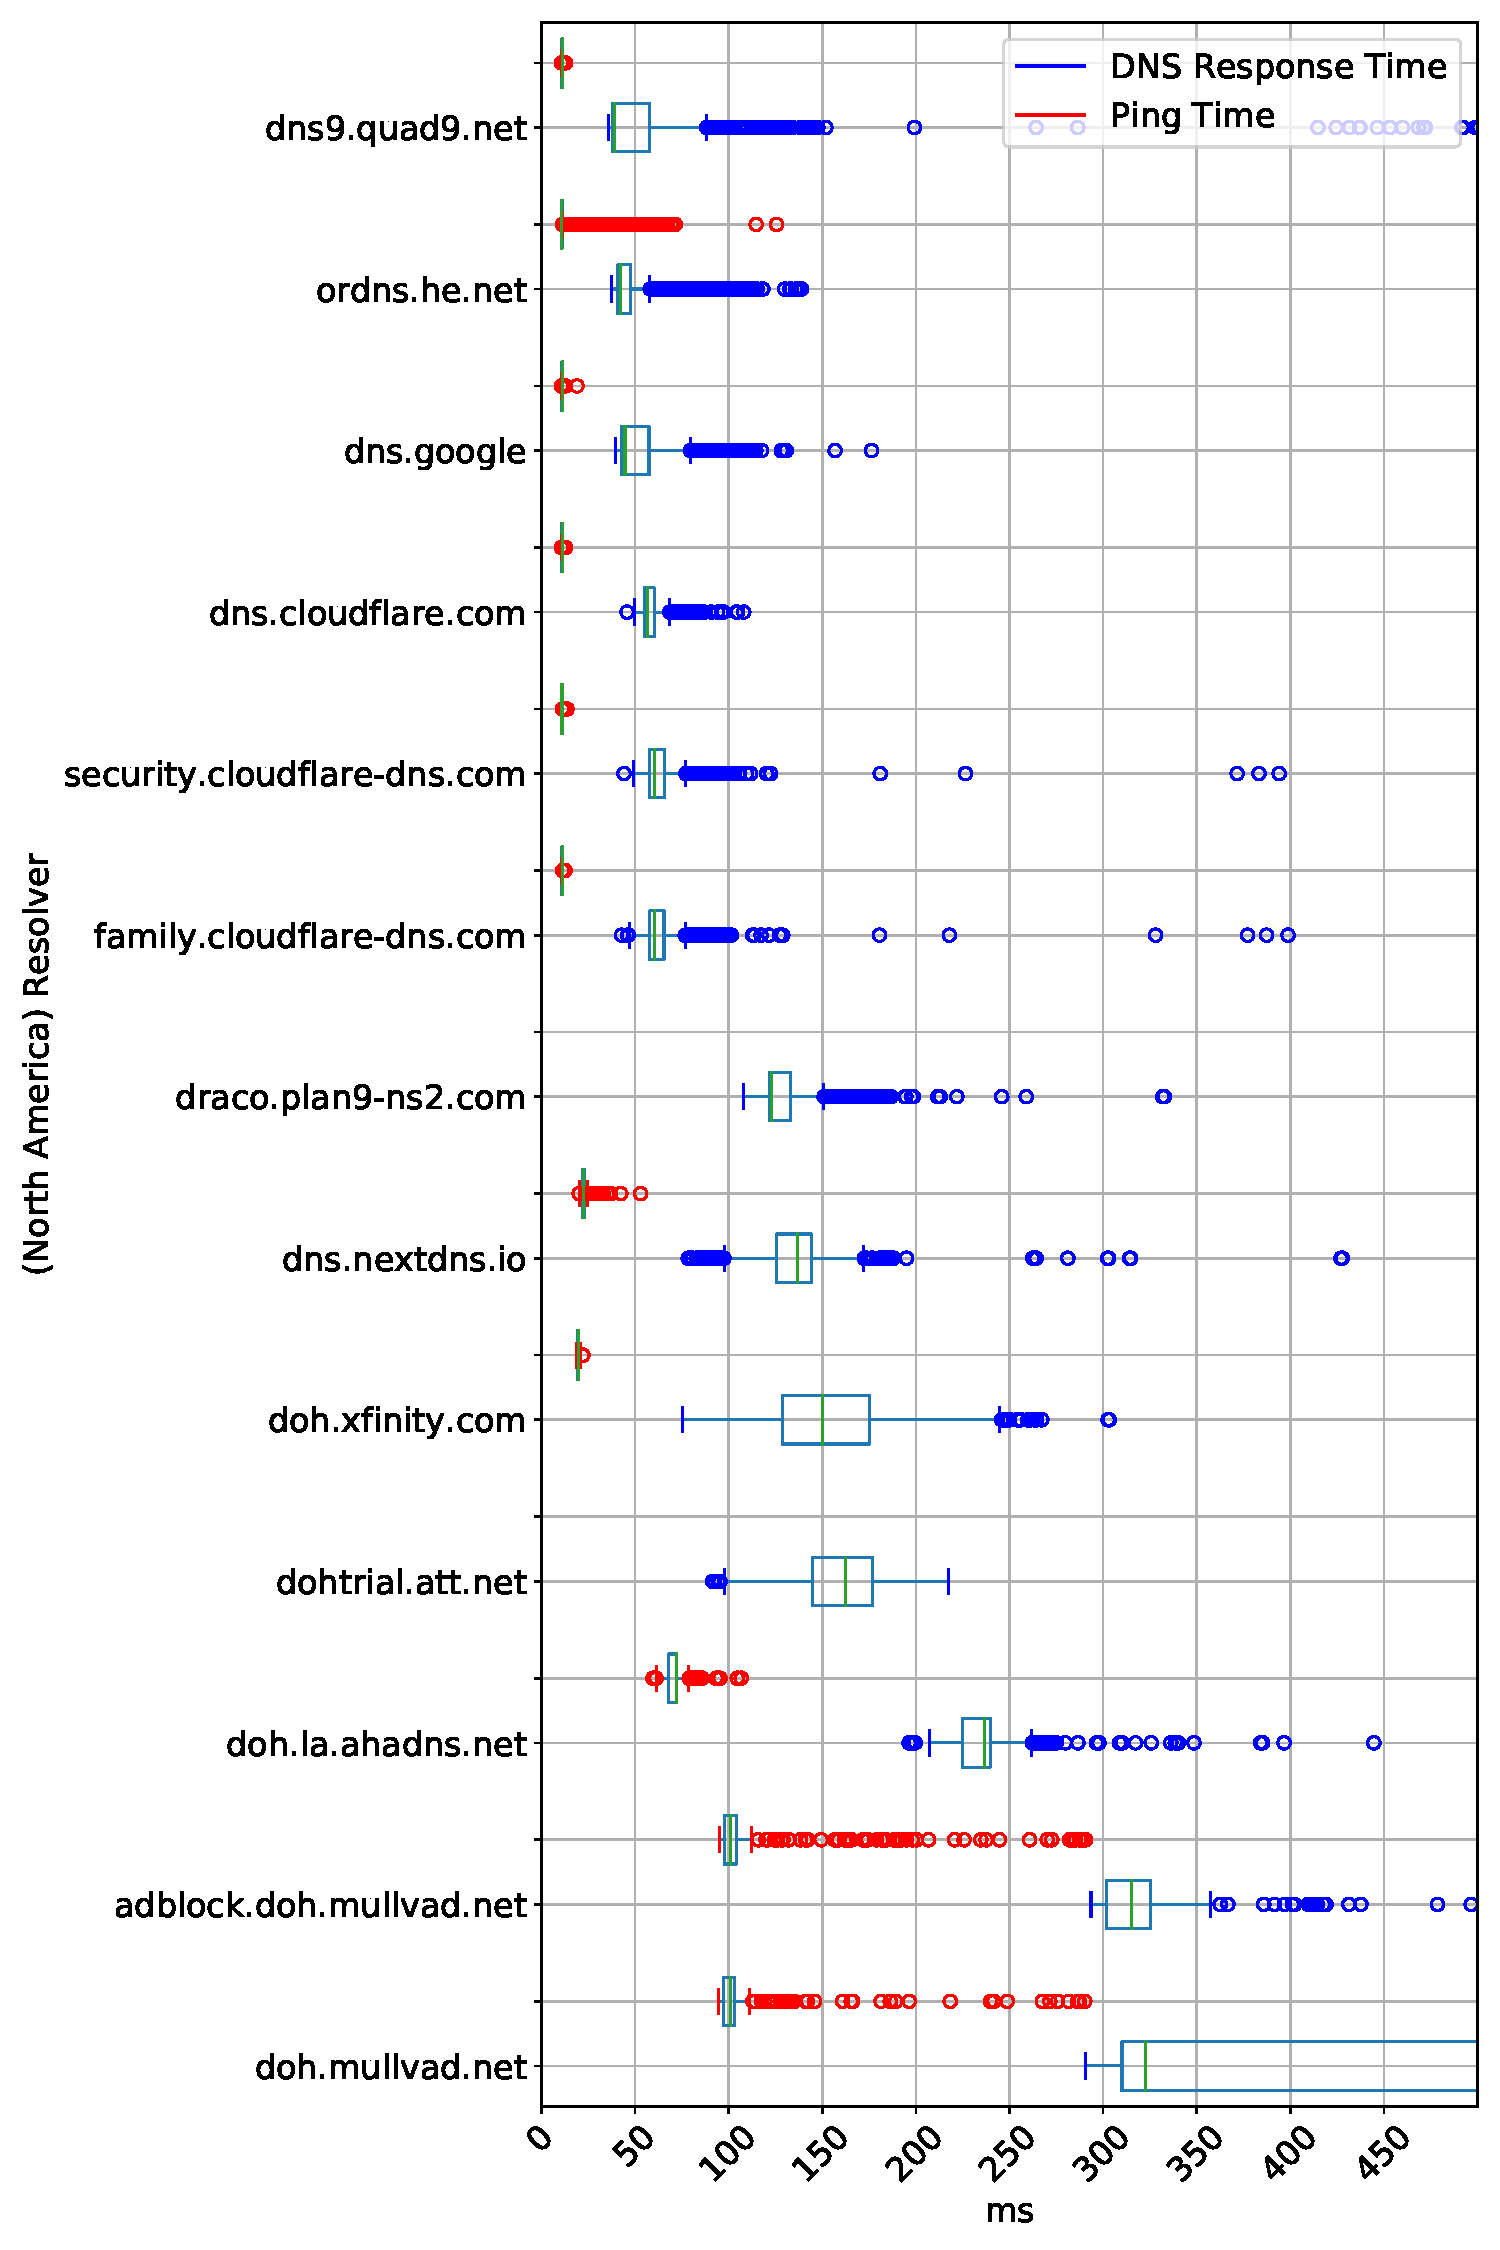
\includegraphics[width=0.32\linewidth]{figures/Ohio_North_America.pdf}}%
\hfill%
\subfigure[Asian resolvers measured from Seoul, South Korea]{%
\label{fig:Local_Seoul_Asia}%
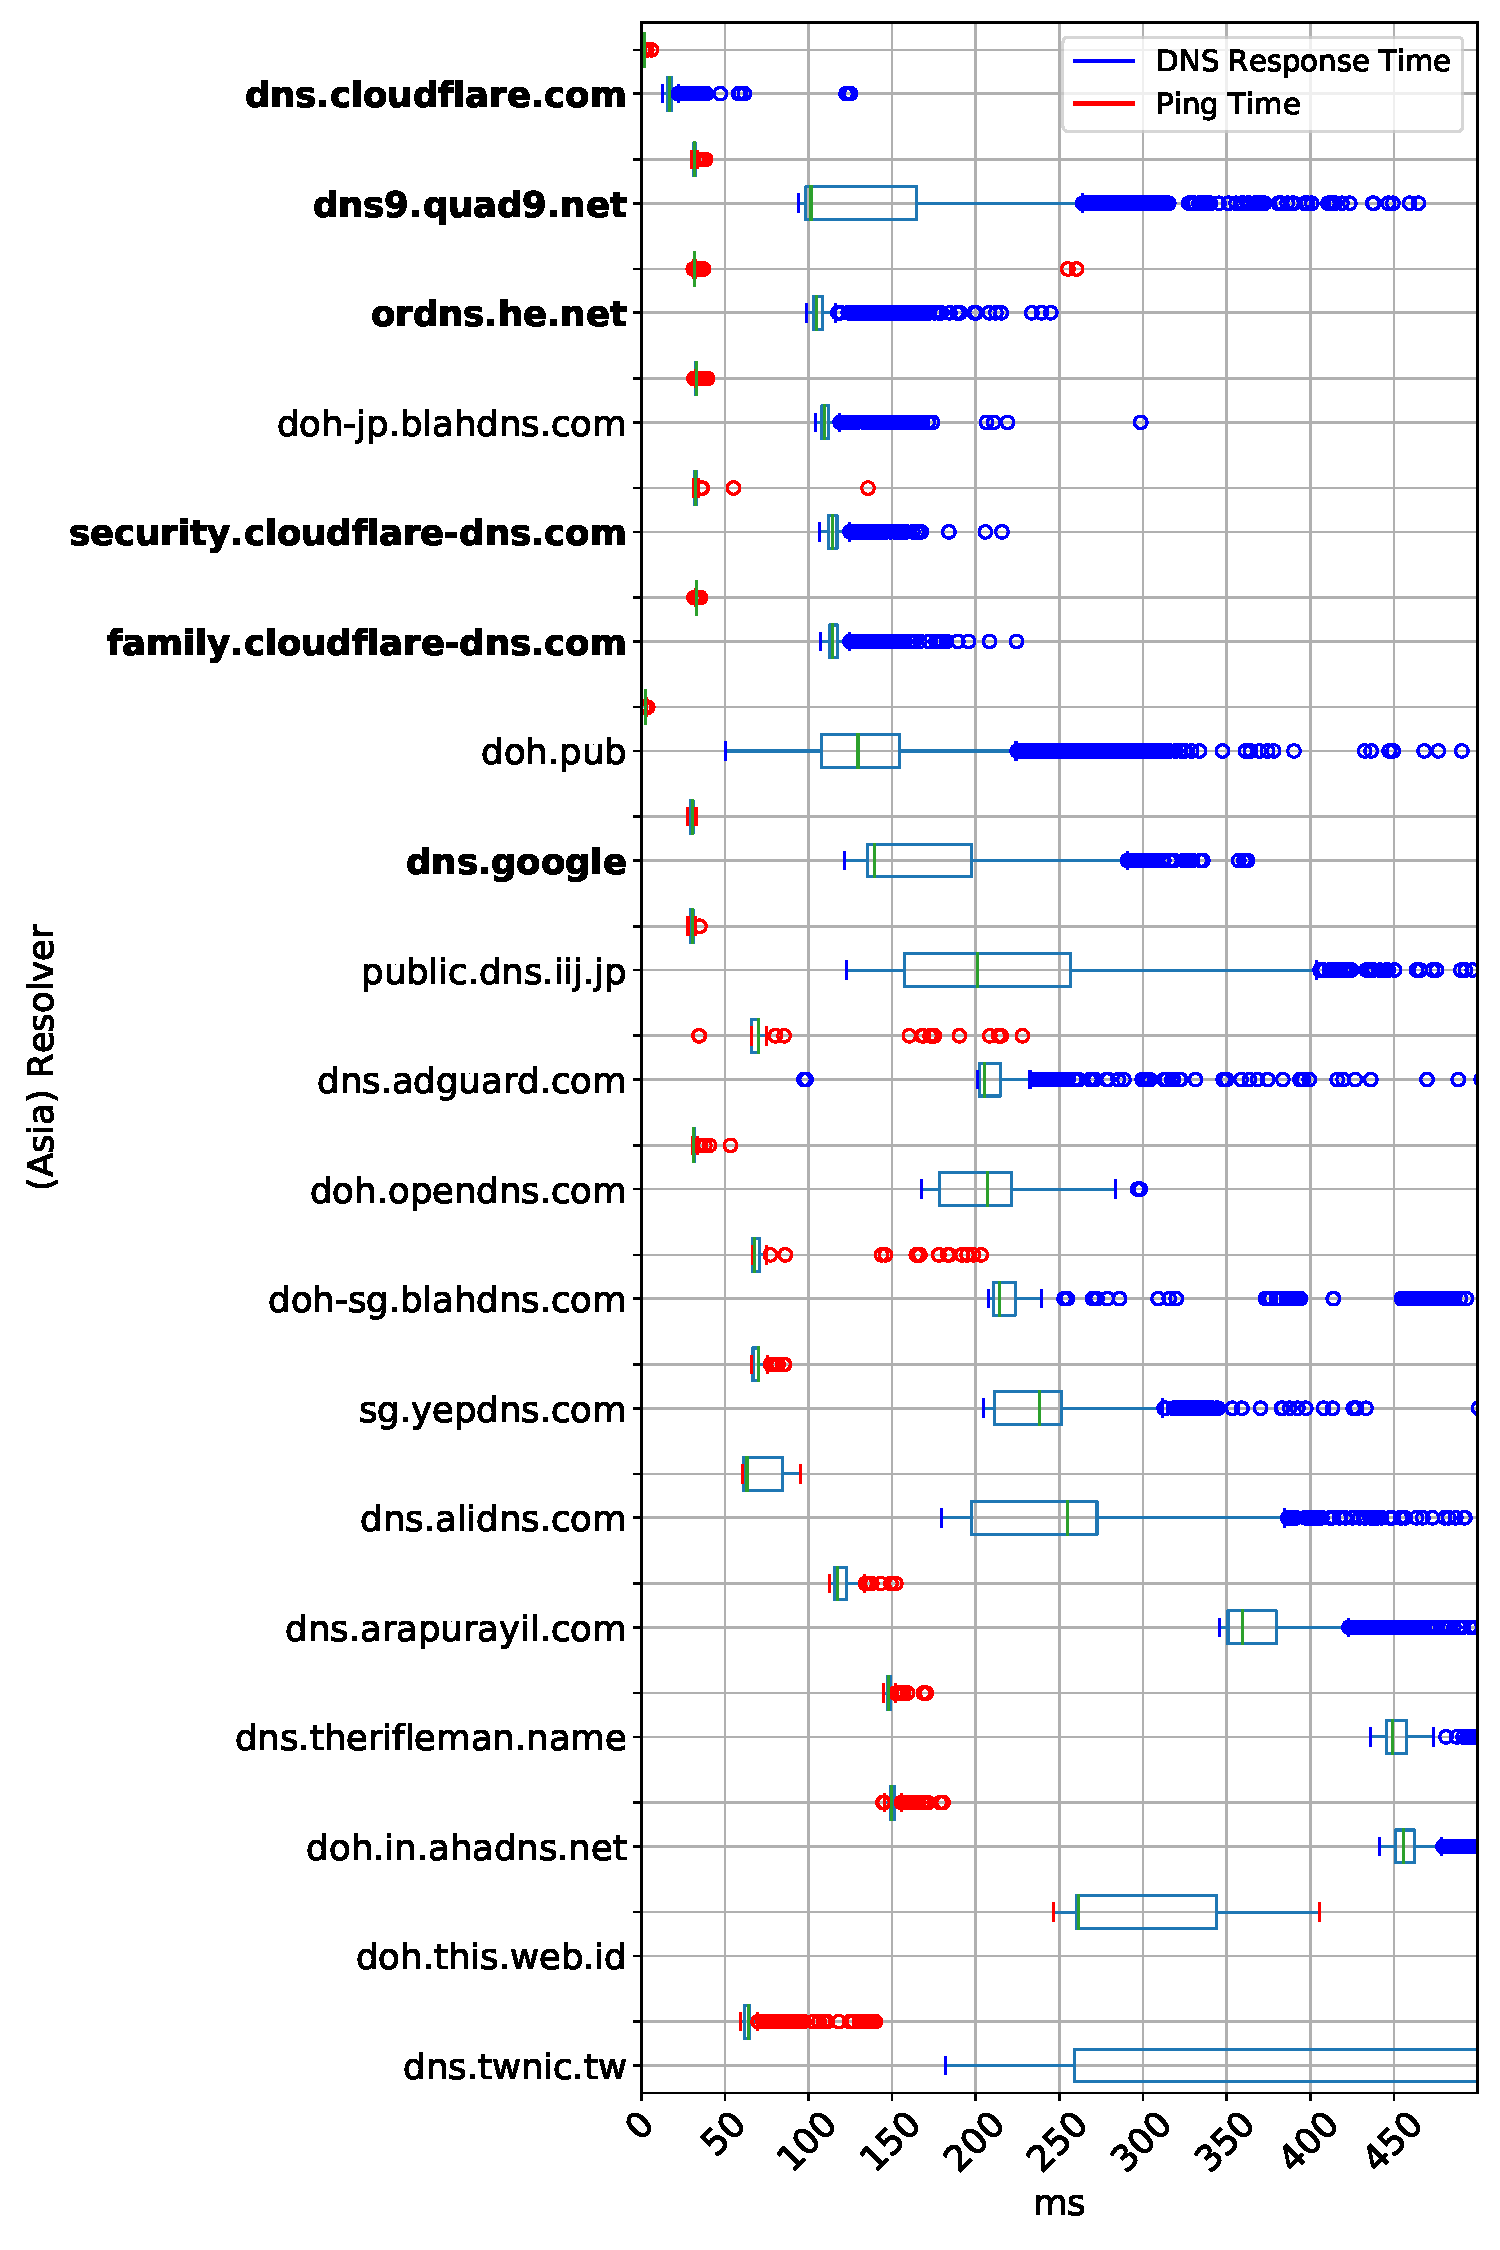
\includegraphics[width=0.32\linewidth]{figures/Seoul_Asia.pdf}}%
\hfill%
\subfigure[European resolvers measured from Frankfurt, Germany]{%
\label{fig:Local_Frankfurt_Europe}%
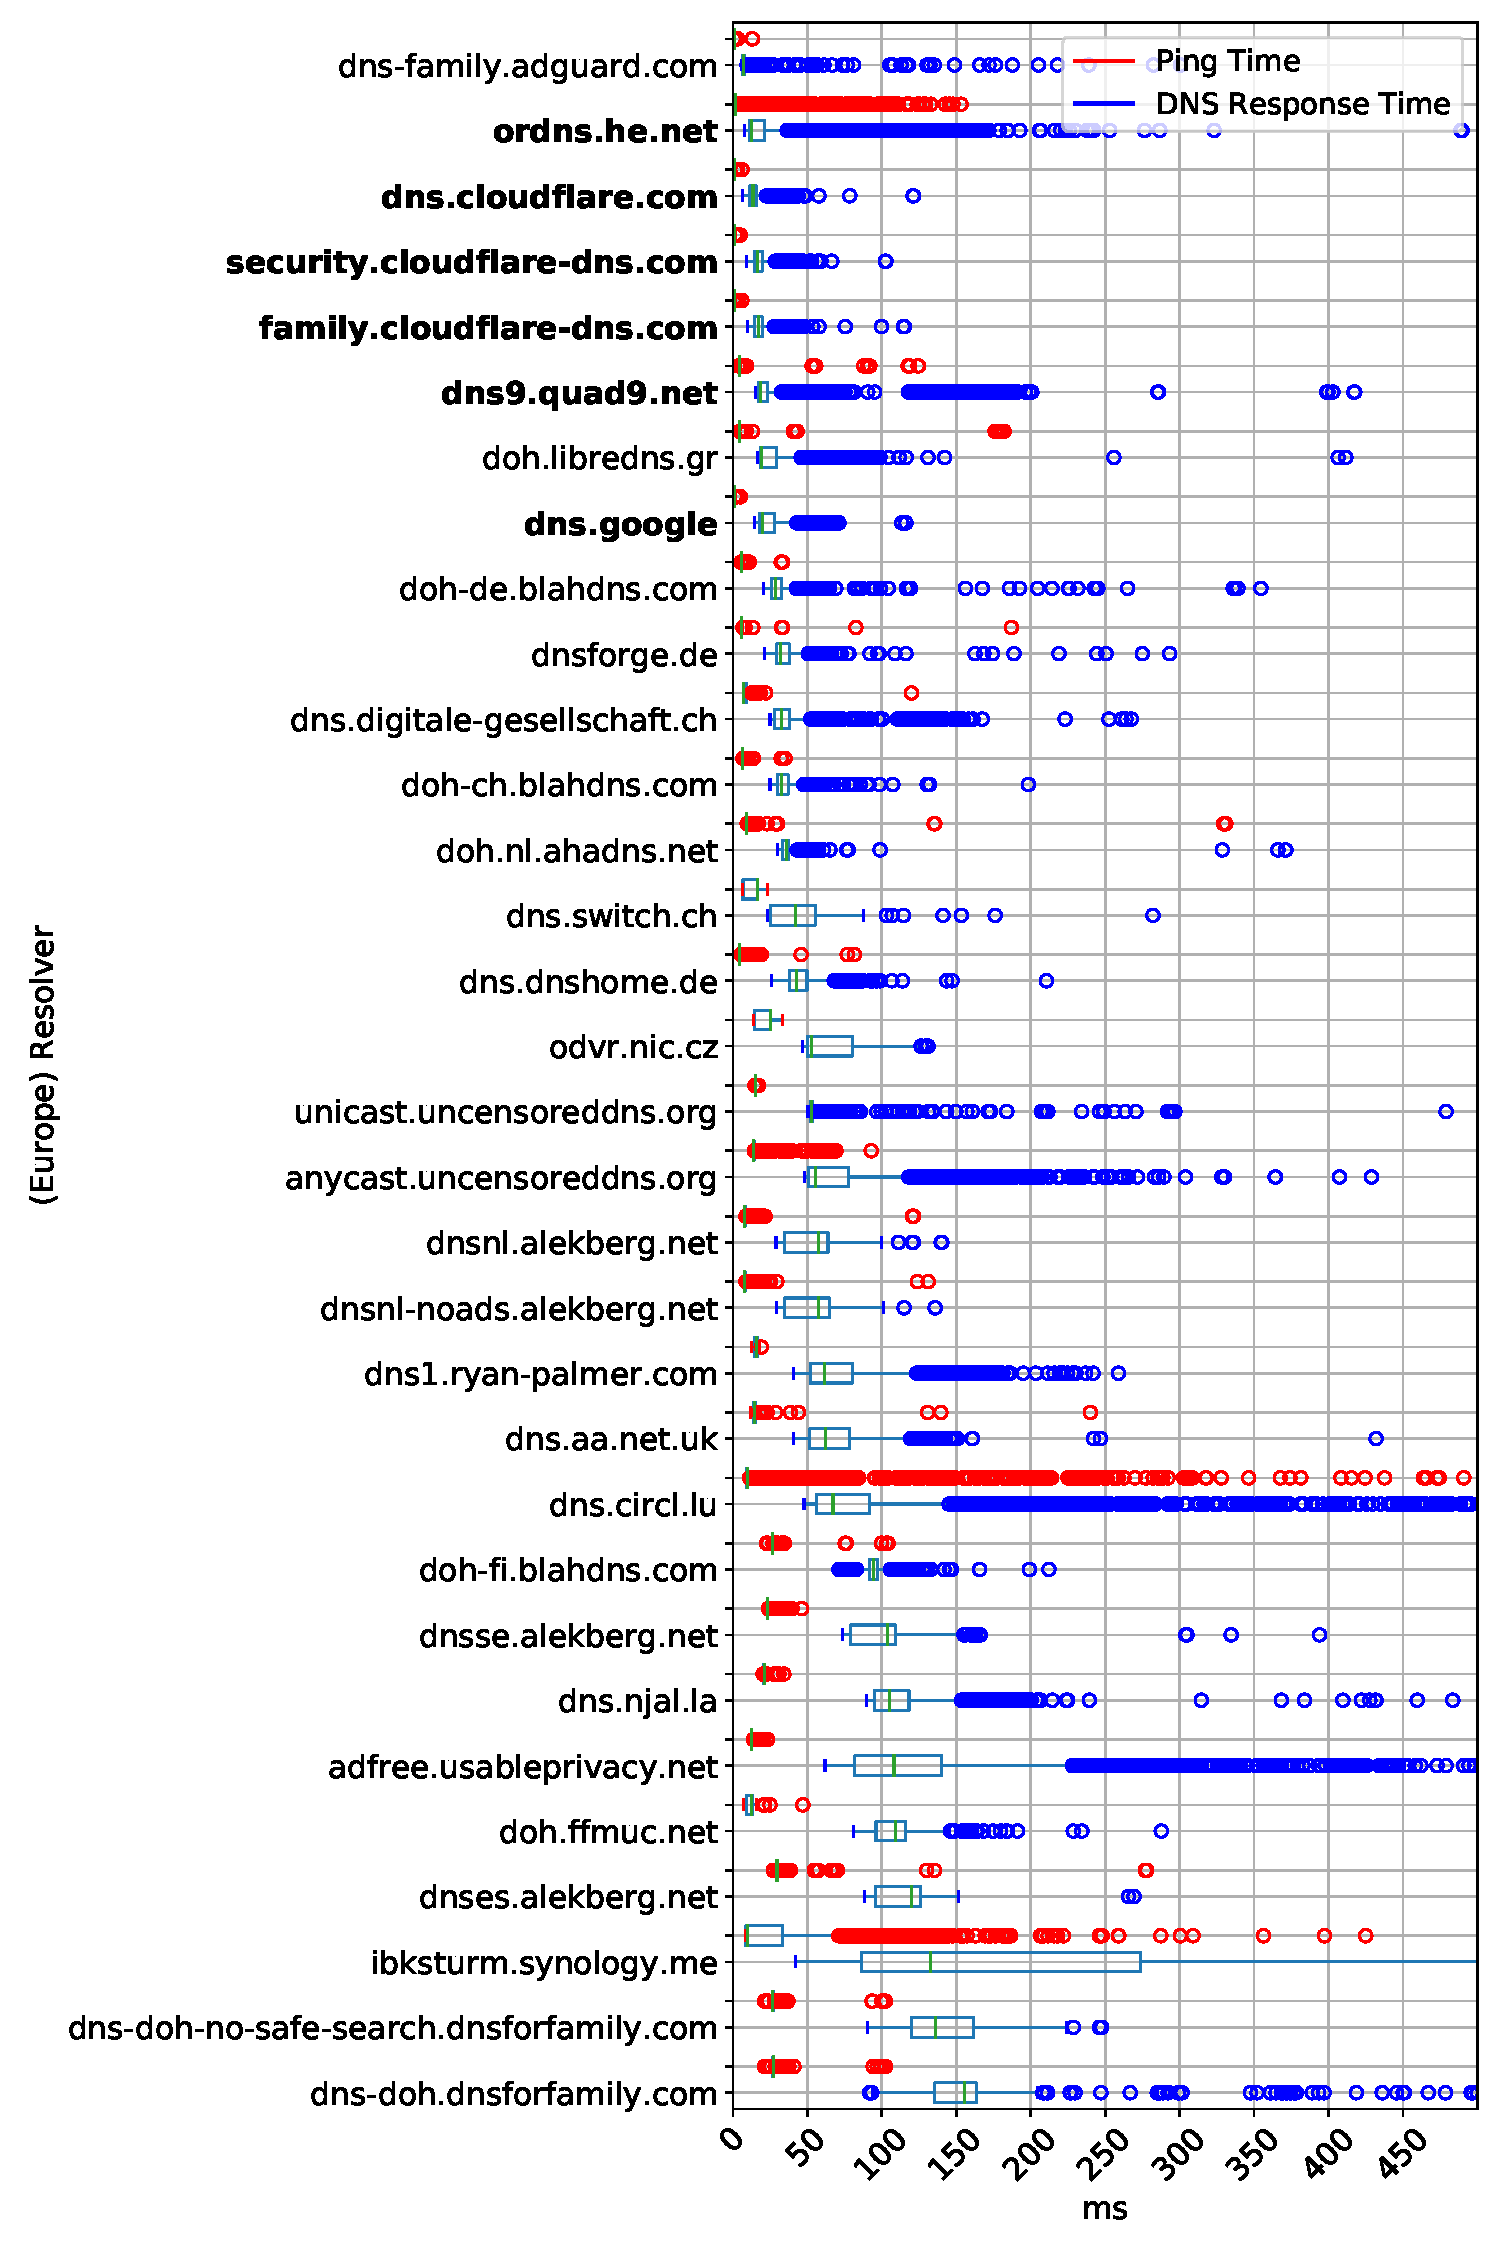
\includegraphics[width=0.32\linewidth]{figures/Frankfurt_Europe.pdf}}%
\caption{Local-to-local resolvers.}
\end{minipage}
\end{figure}
\fi


